\documentclass[11pt]{article}
\usepackage[T1]{fontenc}
\usepackage{lmodern,microtype}
\usepackage[margin=1in]{geometry}
\usepackage{amsmath,amssymb,amsthm,mathtools,booktabs,longtable,array,needspace}
\usepackage{tikz}
\usetikzlibrary{arrows.meta,calc,angles,quotes,patterns,positioning}
\usepackage[hidelinks]{hyperref}
\usepackage[nameinlink,noabbrev]{cleveref}
\hypersetup{pdftitle={A self-contained 0.4144 lower bound for constant-width bodies},pdfsubject={Detailed geometric proof and reproducible finite certificates}}
\allowdisplaybreaks
\setlength{\emergencystretch}{2em}
\numberwithin{equation}{section}
\newtheorem{theorem}{Theorem}[section]
\newtheorem{lemma}[theorem]{Lemma}
\newtheorem{proposition}[theorem]{Proposition}
\newtheorem{corollary}[theorem]{Corollary}
\theoremstyle{definition}\newtheorem{definition}[theorem]{Definition}
\theoremstyle{remark}\newtheorem{remark}[theorem]{Remark}
\newcommand{\R}{\mathbb R}
\newcommand{\Sph}{\mathbb S^2}
\newcommand{\B}{\mathcal B}
\newcommand{\Vol}{\operatorname{Vol}}
\newcommand{\diam}{\operatorname{diam}}
\newcommand{\conv}{\operatorname{conv}}
\newcommand{\tr}{\operatorname{tr}}
\newcommand{\cof}{\operatorname{cof}}
\newcommand{\Qh}{\mathcal Q}
\newcommand{\RJ}{R_{\mathrm J}}
\newcommand{\RS}{R_*}
\newcommand{\VM}{V_{\mathrm M}}
\newcommand{\dd}{\,\mathrm d}
\newcommand{\pp}[1]{[#1]_+}
\newcommand{\ip}[2]{\langle #1,#2\rangle}
\newcommand{\cA}{\mathsf A}
\newcommand{\cH}{\mathsf H}
\newcommand{\mix}{\mathcal V}
\title{\Large\bfseries A self-contained volume bound for bodies of constant width\\[5pt]
\large Circumsphere contacts, compulsory completion, and the constant \(0.4144\)}
\author{}
\date{23 September 2026}
\begin{document}
\maketitle
\begin{abstract}
We give a detailed computer-assisted proof that every convex body in
three-dimensional Euclidean space of constant width $w>0$ has volume strictly
larger than $(259/625)w^3=0.4144w^3$. The proof uses no assumption about
symmetry or a finite generating set of the unknown body. After normalization,
its minimum circumradius divides the argument into two regimes. In the first,
a radial divergence estimate is strengthened on eight disjoint contact caps.
In the second, four circumsphere contacts determine an explicit inner body.
A mixed-volume inequality forces additional volume in every constant-width
completion of that inner body. Opposite contact edges are treated jointly:
a change of normal coordinates cancels midpoint displacement, a convexity
argument controls edge obliquity, and three exact deficit identities couple
the resulting integrals. We develop the necessary support-function and
mixed-volume preliminaries, derive the boundary formulas, and specify every
finite numerical premise and its directed-rounding verification. The code,
rational input data, and freshly recomputed reports accompany this manuscript.
The result is not the sharp Meissner inequality; the remaining losses are
identified at the end.
\end{abstract}
\begingroup
\small
\tableofcontents
\endgroup
\newpage

\section{The theorem and how the proof reaches it}\label{sec:intro}
A convex body is a compact convex subset of $\R^3$ with nonempty interior.
Its width in a unit direction is the distance between the two supporting
planes perpendicular to that direction. A body of constant width $w$ has the
same width in every direction. The three-dimensional Blaschke--Lebesgue
problem asks for the least volume in this class.

\begin{theorem}\label{thm:main}
If $K\subset\R^3$ is a convex body of constant width $w>0$, then
\begin{equation}\label{eq:main}
 \boxed{\Vol(K)>\frac{259}{625}w^3=0.4144w^3.}
\end{equation}
The proof is computer-assisted. Its numerical premises are the three finite
certificates stated and explained in \cref{sec:integralcert,sec:hullcert,sec:radialcert}.
\end{theorem}

The conjectured sharp value is the volume of a Meissner tetrahedron,
\begin{equation}\label{eq:Meissner}
 \VM=\frac{\pi}{12}\left(8-3\sqrt3\arccos\frac13\right)
       =0.419860045965080\ldots
\end{equation}
at width one; see \cite{HyndVolume,Bogosel}. We do not assume this conjecture.
Hyra's posted computation gives the lower bound
$(130838246407123/10^{15})\pi=0.411040473721188\ldots$ \cite{Hyra}.
We use the radial method of that work, with the full derivation and a new
finite set of rational data specified here. The other part of the proof is
a geometric completion estimate. Standard foundations are referenced to
\cite{Schneider}; all identities needed to connect them to our estimate are
derived below.

Dilation multiplies width by $w$ and volume by $w^3$. We therefore work at
width one until the final step. Translate the center of the smallest
containing ball to the origin and call its radius $R$. We will prove
\[
 \frac12\le R\le\RJ:=\sqrt{3/8}.
\]
The exact dividing radius and deficit cutoff are
\begin{equation}\label{eq:cutoffs}
 \RS=\frac{60849}{100000},\qquad A_0=\frac2{25}.
\end{equation}
The final coverage is as follows. Decimals in this table are only readable
summaries of outward-enclosed rational numbers.
\begin{center}
\begin{tabular}{@{}lll@{}}
\toprule
Circumradius & Estimate used & Certified lower value exceeds\\
\midrule
$1/2\le R\le3/5$ & Analytic radial estimate & $0.4173574$\\
$3/5\le R\le\RS$ & Eight rational cap certificates & $0.4144109551797$\\
$\RS\le R\le\RJ$ & Contact hull and completion & $0.4144467$\\
\bottomrule
\end{tabular}
\end{center}

Here is the reason for the split. Near $\RJ$, the contacts of the smallest
sphere are nearly a regular tetrahedron. They provide a useful inner body,
but merely containing this inner body is not the full constant-width
condition. We must also account for volume that a constant-width completion
has to add. Farther from $\RJ$, the radial argument is more effective and
does not require the nearly tetrahedral description.

\begin{figure}[ht]
\centering
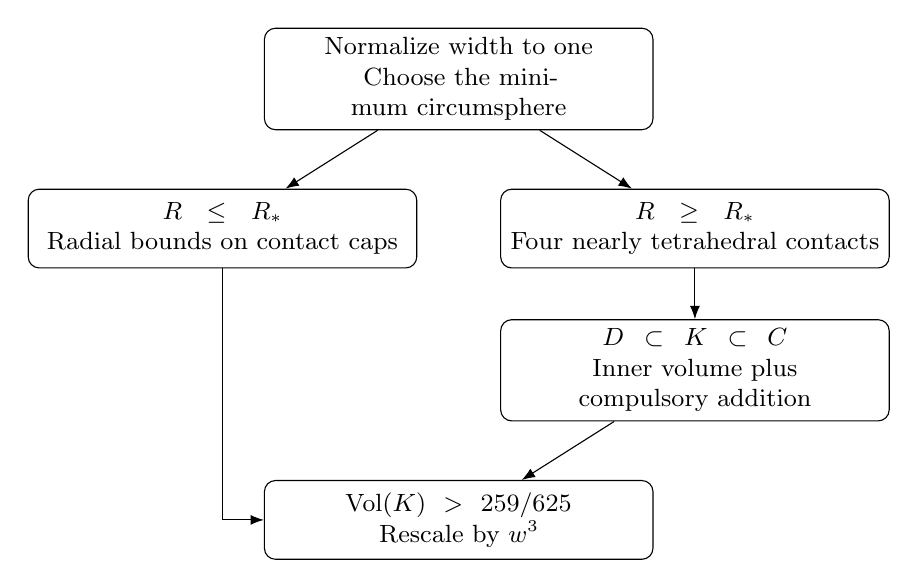
\begin{tikzpicture}[>=Latex, every node/.style={font=\small},
 box/.style={draw,rounded corners,align=center,minimum height=10mm,text width=47mm}]
\node[box] (k) at (0,0) {Normalize width to one\\Choose the minimum circumsphere};
\node[box] (r) at (-3,-1.9) {$R\le R_*$\\Radial bounds on contact caps};
\node[box] (c) at (3,-1.9) {$R\ge R_*$\\Four nearly tetrahedral contacts};
\node[box] (d) at (3,-3.7) {$D\subset K\subset C$\\Inner volume plus compulsory addition};
\node[box] (v) at (0,-5.6) {$\Vol(K)>259/625$\\Rescale by $w^3$};
\draw[->] (k) -- (r);\draw[->] (k) -- (c);\draw[->] (c) -- (d);
\draw[->] (r.south) -- (-3,-5.6) -- (v.west);
\draw[->] (d) -- (v);
\end{tikzpicture}
\caption{The proof has two complementary geometric branches. The numerical
certificates verify explicit inequalities inside these branches; they do not
search over unknown convex bodies.}\label{fig:roadmap}
\end{figure}

\section{Preliminaries: support functions, width, and curvature}\label{sec:prelim}
\subsection{Support functions and containment}
For a nonempty compact convex set $E$ its support function is
\[
 h_E(n)=\max_{x\in E}x\cdot n,\qquad n\in\Sph.
\]
It extends to all of $\R^3$ by positive homogeneity. The intersection of the
half-spaces $x\cdot n\le h_E(n)$ is exactly $E$, by separation. Thus
\begin{equation}\label{eq:supportorder}
 E\subset F\quad\Longleftrightarrow\quad h_E\le h_F.
\end{equation}
The Minkowski sum is $E+F=\{x+y:x\in E,y\in F\}$. Maximizing a linear
functional separately in $x,y$ proves
\[
 h_{E+F}=h_E+h_F,\quad h_{tE}=t h_E\ (t\ge0),\quad h_{-E}(n)=h_E(-n).
\]
We write $B=\{x:|x|\le1\}$. Its support function is the constant one.

\begin{lemma}[Width and opposite points]\label{lem:width}
A convex body has width one if and only if
\begin{equation}\label{eq:width}
 h_K(n)+h_K(-n)=1\quad(n\in\Sph).
\end{equation}
Such a body has diameter one, $K+(-K)=B$, and the following property: if $n$
is an outward unit normal at $x\in\partial K$, then $x-n\in K$.
\end{lemma}
\begin{proof}
The supporting planes have equations $n\cdot x=h_K(n)$ and
$n\cdot x=-h_K(-n)$, proving the width assertion and the Minkowski identity.
For $x,y\in K$, take $n=(x-y)/|x-y|$ when $x\ne y$. Then
$|x-y|\le h_K(n)+h_K(-n)=1$. Conversely, opposite supporting planes have
points of $K$ at projected distance one, so the diameter is one. Finally,
choose $y\in K$ on the plane opposite $x$. The equations
$(x-y)\cdot n=1$ and $|x-y|\le1$ force $x-y=n$.
\end{proof}
The same argument shows that each supporting plane of a constant-width body
has a unique contact point. Uniqueness of the contact point does not mean
that the boundary has a unique normal at every point.

\subsection{The unit-ball transform}
For a nonempty compact set $E$, put
\[
 \B(E)=\bigcap_{e\in E}\overline B(e,1).
\]
This operation reverses inclusion. Also a width-one body obeys
\begin{equation}\label{eq:selfdual}
 K=\B(K).
\end{equation}
Diameter one proves $K\subset\B(K)$. Conversely, if $x\in\B(K)$, choose a
point minimizing $n\cdot y$ on $K$. Then
\[
 n\cdot x\le n\cdot y+|x-y|\le-h_K(-n)+1=h_K(n).
\]
Use \cref{eq:supportorder}. This simple fact will turn an outer approximation
of $K$ into an inner approximation.

\subsection{Mixed volumes and the normalization of the coefficients}
We use the standard three-dimensional mixed volume $\mix(E,F,G)$, symmetric,
continuous, monotone in each argument, and multilinear under Minkowski
addition and nonnegative scaling. Its normalization is
$\mix(E,E,E)=\Vol(E)$. These foundational properties and the surface-area
representation are described in \cite[Chapter 5]{Schneider}.

Steiner's formula, in our normalization, reads
\begin{equation}\label{eq:steiner}
 \Vol(E+tB)=V_E+S_Et+M_Et^2+\frac{4\pi}{3}t^3,
\end{equation}
where $V_E=\Vol(E)$, $S_E$ is surface area,
$S_E=3\mix(E,E,B)$, and $M_E=3\mix(E,B,B)$. In particular $M_E$ is the
coefficient of $t^2$, not the total integral of mean curvature under a
possibly different convention.

\begin{lemma}[Blaschke's identity]\label{lem:blaschke}
For a width-one body,
\begin{equation}\label{eq:blaschke}
 S_K=2V_K+\frac{2\pi}{3},\qquad M_K=2\pi.
\end{equation}
\end{lemma}
\begin{proof}
Set $m=\mix(K,K,-K)$. Reflection invariance gives
$\mix(K,-K,-K)=m$. Expanding $B=K+(-K)$ yields
\[
 \frac{4\pi}{3}=2V_K+6m,\qquad S_K/3=V_K+m.
\]
Eliminate $m$. Also
$2M_K=3\mix(K+(-K),B,B)=3\Vol(B)=4\pi$.
\end{proof}

\subsection{Curvature-radius matrices and support-function integrals}
The spherical gradient and Hessian are taken with respect to the unit-sphere
metric. For a twice differentiable support function $h$, define
\[
 \Qh h=\nabla^2_{\Sph}h+hI
\]
as a symmetric operator on each two-dimensional tangent plane. The support
point is $h(n)n+\nabla h(n)$; differentiating tangentially shows that its
radius matrix is $\Qh h$. Its eigenvalues are the principal radii of
curvature, rather than the principal curvatures.

For a symmetric $2\times2$ matrix $L$, the cofactor is
$\cof L=(\tr L)I-L$. Define the mixed determinant
\[
 D_2(L,N)=\tfrac12\tr(\cof L\,N).
\]
Then
\begin{equation}\label{eq:detpolar}
 \det((1-t)L+tN)=(1-t)^2\det L+2t(1-t)D_2(L,N)+t^2\det N.
\end{equation}
The area formula and the mixed-volume formula are
\begin{equation}\label{eq:supportintegrals}
 S_E=\int_{\Sph}\det\Qh h_E\dd\sigma,\qquad
 3\mix(F,E,E)=\int_{\Sph}h_F\det\Qh h_E\dd\sigma.
\end{equation}
Here $\sigma(\Sph)=4\pi$.

These formulas extend to the bodies below without assuming smooth boundaries.
If $E+F=B$, the distributional matrices $\Qh h_E,\Qh h_F$ are positive
semidefinite measures whose sum is $I\,d\sigma$. Both are therefore bounded
matrix densities between $0$ and $I$. It follows in local coordinates that
$h_E,h_F\in C^{1,1}$; that is, their first derivatives are Lipschitz. The
area measures in \cref{eq:supportintegrals} have the displayed bounded
almost-everywhere densities. Convolution by rotations gives smooth support
functions, preserves inclusion and $E+F=B$, and converges in $C^1$ and in
$W^{2,p}$ for every finite $p$. Consequently the identities used here pass
to the limit. This also applies to $K$ because $K+(-K)=B$.

\begin{lemma}[Two variation identities]\label{lem:variations}
Suppose $D\subset K$ are Minkowski summands of $B$. Put
$f=h_K-h_D$, $\cA=\Qh h_D$, and $\cH=\Qh h_K$. Then
\begin{align}
 3(V_K-V_D)&=\int f[\det\cA+D_2(\cA,\cH)+\det\cH]\dd\sigma,
       \label{eq:volvariation}\\
 2(S_K-S_D)&=\int f(\tr\cA+\tr\cH)\dd\sigma.
       \label{eq:areavariation}
\end{align}
\end{lemma}
\begin{proof}
Let $E_t=(1-t)D+tK$. Multilinearity gives
$\frac{d}{dt}V_{E_t}=\int f\det((1-t)\cA+t\cH)\,d\sigma$.
Integrate \cref{eq:detpolar} over $t\in[0,1]$; all three coefficients
integrate to $1/3$. For area, differentiation and the mixed-area
representation give
$\frac{d}{dt}S_{E_t}=\int f\tr((1-t)\cA+t\cH)\,d\sigma$.
One can also obtain the last equality by integrating the cofactor expression
by parts; $\operatorname{div}\cof(\Qh h)=0$ on the sphere. Integration in $t$
proves \cref{eq:areavariation}. The smoothing argument above covers the
$C^{1,1}$ case.
\end{proof}

\section{The minimum circumsphere and its contact tetrahedron}\label{sec:contacts}
\subsection{Existence and balance}
A smallest closed ball containing $K$ exists by compactness. Put its center at
zero, write its radius as $R$, and let $\mathcal C=K\cap R\Sph$ be its contact
set. Then $0\in\conv\mathcal C$. To prove this, otherwise choose a unit
vector $e$ and $\alpha>0$ with $e\cdot y\ge\alpha$ on all contacts. The
compact subset $\{y\in K:e\cdot y\le\alpha/2\}$ lies strictly inside the
sphere, with maximal radius $\mu<R$ when it is nonempty. For sufficiently
small $t>0$, its points have $|y-te|\le\mu+t<R$, and the remaining points
satisfy $|y-te|^2\le R^2-\alpha t+t^2<R^2$. This contradicts minimality.

Caratheodory's theorem, or affine dependence elimination in $\R^3$, gives a
minimal subset $y_i=Ru_i$, $2\le n\le4$, with
\begin{equation}\label{eq:balance}
 \lambda_i>0,\quad\sum_i\lambda_i=1,\quad\sum_i\lambda_i y_i=0.
\end{equation}
A minimal such subset is affinely independent. The diameter inequalities and
balance imply
\[
 y_i\cdot y_j\ge R^2-\tfrac12,\qquad
 0\ge R^2-\tfrac12(1-\lambda_i).
\]
Thus
\begin{equation}\label{eq:weightbound}
 \lambda_i\le1-2R^2,\qquad
 \frac12\le R\le\RJ=\sqrt{3/8}.
\end{equation}
The lower bound uses diameter one. The upper bound follows by summing the
weight inequalities and using $n\le4$. If $R^2>1/3$, three contacts cannot
have weights summing to one; hence exactly four are needed. Their convex
hull is a tetrahedron containing zero in its interior.

The width identity also gives
\begin{equation}\label{eq:innerouter}
 (1-R)B\subset K\subset RB,
\end{equation}
since $h_K\le R$ implies $h_K\ge1-R$. In particular the circumcenter is an
interior point and the radial function of $K$ is well defined.

\subsection{The total squared-edge deficit}
For four contacts define
\[
 d=\tfrac38-R^2,\qquad e_{ij}=1-|y_i-y_j|^2\ge0,\qquad
 A=\sum_{i<j}e_{ij}.
\]
We keep $A$ for this scalar sum and use bold symbols for curvature matrices.

\begin{lemma}\label{lem:budget}
The contacts satisfy
\begin{equation}\label{eq:budget}
 \boxed{16d\le A\le\frac{16d}{1-8d}.}
\end{equation}
For $R\ge\RS$, in particular, $A<A_0=2/25$.
\end{lemma}
\begin{proof}
Expansion using \cref{eq:balance} gives
$\sum_j\lambda_j|y_i-y_j|^2=2R^2$. Hence
\[
 \lambda_i=\tfrac14+2d-\sum_{j\ne i}\lambda_j e_{ij}.
\]
Sum in $i$ to obtain
\[
 8d=\sum_{i<j}(\lambda_i+\lambda_j)e_{ij}.
\]
The other two weights are each at most $1/4+2d$, so
$\lambda_i+\lambda_j\ge1/2-4d$. This proves the upper bound. For the lower
bound set $\bar y=\frac14\sum_i y_i$. The identity
$\sum_{i<j}|y_i-y_j|^2=4\sum_i|y_i-\bar y|^2$ gives
\begin{equation}\label{eq:centroid}
 R^2=\frac38-\frac A{16}+|\bar y|^2.
\end{equation}
Thus $A\ge16d$. The rational comparison
$16(3/8-\RS^2)/(1-8(3/8-\RS^2))<2/25$ gives the last assertion.
\end{proof}

\subsection{Quantitative geometry without assuming symmetry}\label{sec:gram}
We need to know that the sphere intersections keep the intended incidence.
Here is a convenient quantitative justification. Choose the centered regular
unit tetrahedron with columns
\[
 t_0=\frac{(1,1,1)}{2\sqrt2},\quad
 t_1=\frac{(1,-1,-1)}{2\sqrt2},\quad
 t_2=\frac{(-1,1,-1)}{2\sqrt2},\quad
 t_3=\frac{(-1,-1,1)}{2\sqrt2}.
\]
For its $3\times4$ matrix $T$, $TT^T=I/2$ and
$T^TT=\frac12(I_4-\frac14\mathbf1\mathbf1^T)$. Let $E$ have zero diagonal
and off-diagonal entries $e_{ij}$. Centering the squared-distance matrix
shows that the centered contacts are congruent to
\begin{equation}\label{eq:affineframe}
 y_i-\bar y=(I+Q)^{1/2}t_i,\qquad Q=2TET^T.
\end{equation}
Indeed, the centered Gram matrix is $-\frac12J\mathcal D J$, where
$J=I_4-\mathbf1\mathbf1^T/4$ and $\mathcal D_{ij}=|y_i-y_j|^2$.
Its difference from the regular Gram matrix is $JEJ/2$, which is also
$T^TQT$. This proves \cref{eq:affineframe} up to an orthogonal map.

The contribution of a single $e_{ij}$ to $Q$ is
$2e_{ij}(t_it_j^T+t_jt_i^T)$. Its eigenvalues, on the directions
$t_i-t_j,t_i+t_j$ and their perpendicular, are $-e_{ij},e_{ij}/2,0$.
Therefore
\begin{equation}\label{eq:Qbounds}
 -AI\preceq Q\preceq(A/2)I.
\end{equation}
Let $a_i=\sum_{j\ne i}e_{ij}$. Since $|y_i|=R$, the circumcenter equations
in the centered regular frame give
\[
 (I+Q)^{1/2}(-\bar y)=-\frac14\sum_i a_it_i.
\]
Now $\sum_i a_it_i=\sum_{i<j}e_{ij}(t_i+t_j)$ and
$|t_i+t_j|=1/\sqrt2$. Hence
\begin{equation}\label{eq:centroidbound}
 |\bar y|\le\frac{A}{4\sqrt2\sqrt{1-A}}.
\end{equation}
These estimates imply nondegeneracy for $A\le A_0$. All triangular faces
are acute, because their squared side lengths belong to $[1-A_0,1]$ and
$1<2(1-A_0)$. The centered affine tetrahedron contains a ball of radius
$\sqrt{1-A}/\sqrt{24}$; \cref{eq:centroidbound} is smaller, since
$3A^2<4(1-A)^2$. Thus its circumcenter is interior throughout this whole
six-dimensional deficit region. Its circumradius is at most
\begin{equation}\label{eq:circcontrol}
 \sqrt{3/8}\sqrt{1+A/2}+\frac{A}{4\sqrt2\sqrt{1-A}}<1.
\end{equation}
The final comparisons hold already at $A=A_0$ and are rechecked in
\path{verification/verify_auxiliary.py}. These statements concern all six
edge deficits, not a chosen symmetric family.

\section{A forced inner body and its complementary outer body}\label{sec:duality}
For the selected four contacts let
\begin{equation}\label{eq:CD}
 Y=\{y_0,y_1,y_2,y_3\},\qquad C=RB\cap\B(Y),\qquad D=\B(C).
\end{equation}
The constraints $Y\subset K$ and $K\subset RB$ give $K\subset C$. Applying
the order-reversing transform and \cref{eq:selfdual} gives
\begin{equation}\label{eq:containment}
 \boxed{D\subset K\subset C.}
\end{equation}
Both $C$ and $D$ have interior. The first contains $(1-R)B$; the second
contains $(1-R)B$ because $C\subset RB$. The point of $D$ is that it is
forced by the four contact locations and $R$, without knowing the rest of
$K$. It usually does not have constant width.

\begin{lemma}[Complementarity of intersections of small balls]\label{lem:complement}
Suppose $C$ is a full-dimensional finite intersection of closed balls whose
radii $r_i$ satisfy $0<r_i\le1$, and $D=\B(C)$ is nonempty. Then
\begin{equation}\label{eq:complement}
 C+(-D)=B,\qquad h_C(n)+h_D(-n)=1.
\end{equation}
\end{lemma}
\begin{proof}
Fix a support point $x\in C$ with outward unit normal $n$. An interior point
of $C$ is strictly inside every defining ball. The normal cone of this
strictly feasible intersection is therefore the cone generated by the active
ball normals. Explicitly,
\[
 n=\sum_i a_i\frac{x-c_i}{r_i},\qquad a_i\ge0,\qquad |x-c_i|=r_i
\]
over the active indices. To recall the elementary justification, if $n$ were
outside that finitely generated cone, a separating direction, made slightly
strict by adding a direction toward an interior point, would decrease all
active constraints and increase $n\cdot x$. Small displacement in that
direction would contradict support maximality. This proves the cone formula.

Since the active normals are unit, $\sum_i a_i\ge1$. Expanding the ball
inequality at any $z\in C$ gives
\[
 \frac{x-c_i}{r_i}\cdot(z-x)\le-\frac{|z-x|^2}{2r_i}.
\]
Consequently
\[
 |z-(x-n)|^2
 =1+|z-x|^2+2n\cdot(z-x)
 \le1+\left(1-\sum_i\frac{a_i}{r_i}\right)|z-x|^2\le1.
\]
Thus $x-n\in D$. On the other hand, for any $y\in D$, $|x-y|\le1$, so
$n\cdot x-n\cdot y\le1$. The choice $y=x-n$ attains equality. This is
$h_C(n)+h_D(-n)=1$, and equality of support functions proves the Minkowski
identity.
\end{proof}

The lemma applies to \cref{eq:CD}: the defining radii are one and $R<1$.
It provides substantially more information than $D\subset K\subset C$.
In particular both $C$ and $D$ are summands of the unit ball, so all the
curvature formulas of \cref{sec:prelim} apply.

\begin{lemma}[Complementary volume and area identities]\label{lem:dualvol}
With the notation of \cref{eq:steiner},
\begin{equation}\label{eq:dualvol}
 \boxed{V_D=\frac{4\pi}{3}-M_C+S_C-V_C,\qquad
 S_D=4\pi-2M_C+S_C.}
\end{equation}
Also $M_C+M_D=4\pi$.
\end{lemma}
\begin{proof}
The identity $B=C+(-D)$ allows the formal multilinear substitution
$-D=B-C$. Expanding the cubic volume polynomial gives
\[
 V_D=\Vol(B)-3\mix(C,B,B)+3\mix(C,C,B)-V_C.
\]
Expanding $3\mix(B-C,B-C,B)$ gives the area formula, since simultaneous
reflection leaves $B$ invariant. Finally $M_E=\int h_E\,d\sigma$, so the
support identity gives $M_C+M_D=4\pi$. The formal subtraction is just a
convenient notation for rearranging a polynomial identity between actual
Minkowski sums; no set difference is being assigned a mixed volume.
\end{proof}

\section{The geometry of the circumsphere-clipped intersection}\label{sec:clipgeometry}
This section justifies exactly which surfaces and edges must be integrated.
We work with four balanced contacts and $A\le A_0$. Initially assume all
six $e_{ij}$ are positive; zero deficits will follow by continuity.

\subsection{Why the original vertices are removed by clipping}
Consider the triangular face opposite $y_l$. Give its plane an inward unit
normal $n_l$ and equation $n_l\cdot y=b_l$. The origin is interior, so
$b_l<0<n_l\cdot y_l$. Balance gives
\[
 b_l=-\frac{\lambda_l}{1-\lambda_l}\,n_l\cdot y_l.
\]
Positivity of the incident deficits in the weight equation makes
$\lambda_l<1-2R^2$. As $n_l\cdot y_l\le R$, this implies
\begin{equation}\label{eq:planeheight}
 b_l>R-\frac1{2R}.
\end{equation}
The three vertices of the face lie in $RS^2$. Their planar circumcenter is
$b_ln_l$ and their circumradius squared is $R^2-b_l^2$. Hence the two
intersections of their unit spheres are
\[
 x_l^\pm=\left(b_l\pm\sqrt{1-R^2+b_l^2}\right)n_l.
\]
The plus coefficient is positive. A direct rearrangement shows
$|x_l^+|>R$ if and only if \cref{eq:planeheight} holds. For the minus
coefficient, $|x_l^-|>\sqrt{1-R^2}$ and $x_l^-\cdot y_l<0$, so
$|x_l^--y_l|^2>1$. Thus that intersection is excluded by the fourth ball.
There is no triple intersection of unit spheres in $RB$.

\subsection{The two kinds of circular edges}
Fix an edge of the contact tetrahedron, of length $s=|y_i-y_j|$. Its midpoint
$o=(y_i+y_j)/2$ is perpendicular to $y_i-y_j$, because $|y_i|=|y_j|=R$.
The intersection of the two unit spheres is a circle with
\begin{equation}\label{eq:loadingcircle}
 r=\sqrt{1-s^2/4},\qquad m=|o|=\sqrt{R^2-s^2/4}.
\end{equation}
Write a point on it as $x=o+r v$, $v\perp(y_i-y_j)$ and $|v|=1$.
The clipping condition $|x|\le R$ is
\[
 v\cdot\frac{-o}{m}\ge\frac{1-s^2/2}{2rm}.
\]
Thus the surviving short arc is centered in direction $-o$ and has angular
length
\begin{equation}\label{eq:phi}
 \phi=2\beta,\qquad
 \beta=\arccos\frac{1-s^2/2}{2rm}.
\end{equation}
It is nondegenerate because
\[
 4r^2m^2-(1-s^2/2)^2=R^2(4-s^2)-1
 \ge\frac18-\frac{3A_0}{16}>0,
\]
using $R^2\ge3/8-A/16$ from \cref{eq:centroid}. We call these six arcs the
\emph{unit--unit edges}.

\begin{figure}[ht]
\centering
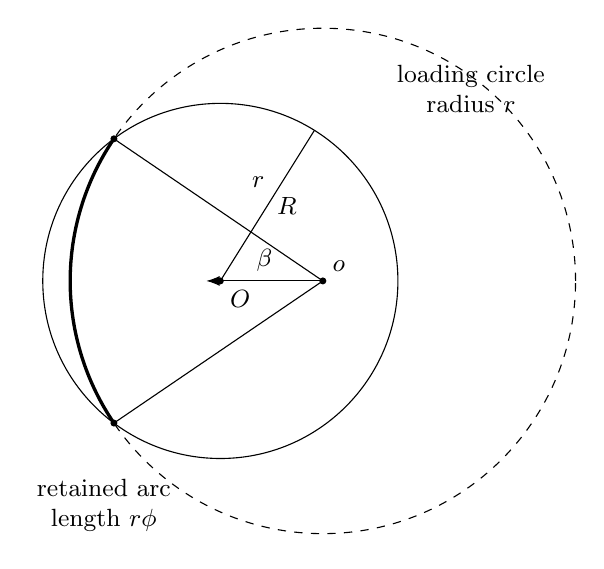
\begin{tikzpicture}[scale=3.7,>=Latex,every node/.style={font=\small}]
\pgfmathsetmacro{\RR}{0.6095}
\pgfmathsetmacro{\ss}{\RR*sqrt(8/3)}
\pgfmathsetmacro{\mm}{sqrt(\RR*\RR-\ss*\ss/4)}
\pgfmathsetmacro{\rr}{sqrt(1-\ss*\ss/4)}
\pgfmathsetmacro{\bb}{acos((1-\ss*\ss/2)/(2*\rr*\mm))}
\draw[thin] (0,0) circle (\RR);
\draw[dashed] (\mm,0) circle (\rr);
\coordinate (o) at (\mm,0);
\coordinate (P) at ({\mm+\rr*cos(180-\bb)},{\rr*sin(180-\bb)});
\coordinate (Q) at ({\mm+\rr*cos(180+\bb)},{\rr*sin(180+\bb)});
\draw[very thick] (P) arc[start angle={180-\bb},end angle={180+\bb},radius=\rr];
\draw[thin] (o)--(P) (o)--(Q);
\draw[->] (o)--({\mm-0.40},0);
\fill (0,0) circle(0.012) node[below right] {$O$};
\fill (o) circle(0.012) node[above right] {$o$};
\fill (P) circle(0.012);\fill (Q) circle(0.012);
\draw[thin] (0,0)--({\RR*cos(58)},{\RR*sin(58)}) node[midway,right] {$R$};
\node at (0.13,0.34) {$r$};
\node at ({\mm-0.20},0.07) {$\beta$};
\node[align=center] at (0.86,0.66) {loading circle\\radius $r$};
\node[align=center] at (-0.40,-0.77) {retained arc\\length $r\phi$};
\end{tikzpicture}
\caption{A section in the loading-circle plane, perpendicular to $y_i-y_j$.
The solid circle is the circum-ball section and the dashed circle is the
intersection of the two unit spheres. The thick inward arc survives clipping.
The displayed scale is illustrative; \cref{eq:loadingcircle,eq:phi} are exact.}
\label{fig:clip}
\end{figure}

There are also edges where a unit sphere meets $RS^2$. Put
\begin{equation}\label{eq:kappagamma}
 \kappa=\sqrt{1-\frac1{4R^2}},\qquad
 \gamma=\arccos\frac1{2R},\qquad d_R=R-\frac1{2R}.
\end{equation}
The intersection of $S(y_i,1)$ and $RS^2$ is the circle of radius $\kappa$
with center $d_R y_i/R$. On that circle another ball, centered at $y_j$,
removes an angular interval of length $2\Psi$, where
\begin{equation}\label{eq:Psi}
 \Psi=\arccos\frac{(1-2R^2)s}{4R\kappa m}.
\end{equation}
For a derivation, write $x=d_Ry_i/R+\kappa v$, $v\perp y_i$, $|v|=1$.
The projection of $y_j$ onto $y_i^\perp$ has length $sm/R$.
The inequality $|x-y_j|\le1$ becomes
\[
 v\cdot\frac{\operatorname{proj}_{y_i^\perp}y_j}{sm/R}
 \ge \frac{d_Rs}{2\kappa m}.
\]
The right side is negative. The excluded interval, centered in the opposite
direction, has half-angle $\arccos(-d_Rs/(2\kappa m))$, which is
\cref{eq:Psi}. We call the surviving arcs the \emph{unit--$R$ edges}.

\subsection{Why the same boundary description holds throughout the domain}
The un-clipped four-ball intersection has tetrahedral incidence at regularity.
Along any path in the positive deficit simplex, \cref{eq:Qbounds,eq:circcontrol}
rule out a degenerate contact tetrahedron or tangent triples of unit spheres.
The preceding argument excludes a unit-sphere triple meeting $RB$, while
\cref{eq:phi} excludes tangency of two unit spheres with the $R$-sphere.
Thus the incidence of the clipped arcs cannot change.

For a starting configuration take a uniformly shrunken regular tetrahedron,
of side $l<1$ close to one and circumradius $\sqrt{3/8}\,l$. The inward
midpoint of a clipped loading arc has squared distance
\[
 1+l^2/2-\sqrt2\,l\sqrt{1-l^2/4}<1
\]
from either of the other two centers. No third sphere crosses the arc, so
its whole relative interior is in the other balls. Connectedness and the
absence of crossing events extend this conclusion to the full domain.
Equivalently, the forbidden caps on $RS^2$ overlap pairwise but have no triple
interior intersection. The surviving regions on $RS^2$ are four spherical
triangles.

The boundary consequently has the following pieces:
\begin{center}
\begin{tabular}{@{}lrl@{}}
\toprule
Piece & Number & Supporting surface\\
\midrule
Hexagonal faces & 4 & Unit spheres\\
Triangular faces & 4 & Sphere of radius $R$\\
Unit--unit edges & 6 & Circles of radius $r$\\
Unit--$R$ edges & 12 & Circles of radius $\kappa$\\
Vertices & 12 & Two unit spheres and the $R$-sphere\\
\bottomrule
\end{tabular}
\end{center}
The Euler check is $12-18+8=2$. Zero deficits may collapse some of the new
arcs. Shrinking all contact positions slightly makes all deficits positive,
retains balance, and converges back to the original configuration. Continuity
of support functions, volumes, and the displayed formulas includes all such
boundary cases. No generic-position assumption is made in the final theorem.

\section{Derivation of the clipped volume formulas}\label{sec:volformula}
We now compute the two terms $V_C,V_D$ explicitly. The calculation is local
along edges, which is why it separates into six scalar functions.

\subsection{Angles at a clipped vertex}
Let $x\in S(y_i,1)\cap S(y_j,1)\cap RS^2$. Its three outward unit normals are
\[
 n_i=x-y_i,\qquad n_j=x-y_j,\qquad n_R=x/R.
\]
Their scalar products are
\[
 n_i\cdot n_j=1-s^2/2,\qquad
 n_i\cdot n_R=n_j\cdot n_R=1/(2R).
\]
Projecting the two other normals into the tangent plane of a face gives
its exterior corner angle. Thus each unit face has corner angle $U$, and the
$R$-face has angle $V$, where
\begin{equation}\label{eq:UV}
 U=\arccos\frac{s}{4Rr\kappa},\qquad
 V=\arccos\left(1-\frac{s^2}{2\kappa^2}\right).
\end{equation}
For example, on the unit face the cosine is
\[
 \frac{(1/(2R))(1-(1-s^2/2))}
 {\sqrt{1-(1-s^2/2)^2}\sqrt{1-1/(4R^2)}}
 =\frac{s}{4Rr\kappa}.
\]
This also fixes which supplementary angle is intended.

Let $\Phi_R$ be the total angular length of the unit--$R$ arcs. Start with
four complete circles, of total angular length $8\pi$. For each pair $ij$,
the forbidden interval $2\Psi_{ij}$ is removed from both circles. There
are no overlapping removals on a single circle, by the no-triple-cap property.
Hence
\begin{equation}\label{eq:PhiR}
 \Phi_R=8\pi-4\sum_{i<j}\Psi_{ij}.
\end{equation}

\subsection{Gauss--Bonnet with all signs and multiplicities}
For a disk-like region on a sphere of radius $a$, with positively oriented
piecewise smooth boundary, Gauss--Bonnet reads
\[
 \frac{\operatorname{area}(F)}{a^2}
 +\int_{\partial F}k_g\dd s+\sum\text{exterior corner angles}=2\pi.
\]
The geodesic curvature $k_g$ is signed according to the interior of the region.
This is especially important on the $R$-sphere, where one of the signed
coefficients below is negative.

Let $S_1$ be the total area of the four unit faces, and $S_R$ that of the
four $R$-faces. At the two endpoints of edge $ij$, the two unit faces each
contribute $U$, giving $4U$ in the sum over all faces. The two $R$-corners
give $2V$. A unit--unit edge contributes geodesic-curvature integral
$(s/2)\phi$ on each of its two unit faces, hence $s\phi$ in total.
A unit--$R$ edge of angular length $\omega$ contributes $\omega/(2R)$ on
its unit face. On the $R$-face the signed contribution is
$(1-1/(2R^2))\omega$: its supporting plane has signed height $d_R$, and
$d_R/R=1-1/(2R^2)$. Consequently
\begin{align}
 S_1&=8\pi-4\sum U-\sum s\phi-\frac{\Phi_R}{2R},\label{eq:S1}\\
 S_R&=R^2\left[8\pi-2\sum V-
                   \left(1-\frac1{2R^2}\right)\Phi_R\right].\label{eq:SR}
\end{align}
Every sum over an unlabeled edge quantity in this section is over the six
unordered contact pairs $i<j$.

\subsection{Volume from boundary vector areas}
The divergence theorem gives $3V_C=\int_{\partial C}x\cdot n\,dA$.
On a unit face centered at $y_i$, $x=y_i+n$, so its contribution is its area
plus $y_i\cdot\int n\,dA$. On an $R$-face it is $R$ times its area.
The vector-area identity
\begin{equation}\label{eq:vectorarea}
 \int_F n\dd A=\frac12\int_{\partial F}n\times\dd n
\end{equation}
holds on a unit sphere. It follows, for instance, componentwise from Stokes'
theorem applied to the constant-coordinate area forms. This is the same
boundary-integral mechanism used for ball-polyhedron volumes in
\cite{HyndVolume}; the following edge contributions are derived for the
present clipped geometry.

For a unit--unit edge let $k=(y_j-y_i)/s$, write $x=o+r v$, and choose the
orientation $\dot v=k\times v$. On the face centered at $y_i$,
$n=(s/2)k+rv$, and
\[
 \int n\times\dd n=(s/2)k\times\Delta x+r^2k\phi.
\]
The neighboring face has the reverse boundary orientation and normal
$-(s/2)k+rv$. Multiplying each vector area by its sphere center and adding
leaves
\[
 -\frac12sr^2\phi+\frac12\det(y_i,y_j,\Delta x).
\]
The endpoints on the $R$-sphere satisfy
\[
 \det(y_i,y_j,\Delta x)=2srm\sin(\phi/2)
   =s\sqrt{R^2(4-s^2)-1}=:T_e.
\]
The sign is positive for the orientation just fixed; the short inward arc
makes this explicit in the loading-circle plane.

For a unit--$R$ edge, use axis $k=y_i/R$ and write its unit-face normal as
$n=-k/(2R)+\kappa v$. The orientation with the unit face on the left is the
negative angular orientation about $k$. Dotting \cref{eq:vectorarea} with
$y_i=Rk$ gives $-R\kappa^2\omega/2$. Summing these contributions proves
\begin{equation}\label{eq:VCledger}
 3V_C=S_1+RS_R-\frac12\sum sr^2\phi+\frac12\sum T_e
                         -\frac12R\kappa^2\Phi_R.
\end{equation}

\subsection{The quadratic Steiner coefficient}
For a piecewise smooth convex boundary, the $t^2$ coefficient in its outer
parallel volume consists of the integrated mean curvature of its smooth
faces and half the exterior angle times edge length. A spherical face of
radius $a$ contributes its area divided by $a$. Along a unit--unit edge,
the angle between outward normals is $2\arcsin(s/2)$, so its contribution
is $r\phi\arcsin(s/2)$. Along a unit--$R$ edge it is $\gamma$, giving
$\kappa\omega\gamma/2$. Vertex neighborhoods first contribute to the
coefficient of $t^3$. Thus
\begin{equation}\label{eq:MCledger}
 M_C=S_1+\frac{S_R}{R}+\sum r\phi\arcsin(s/2)
                         +\frac12\kappa\gamma\Phi_R.
\end{equation}
The coefficients can also be obtained by integrating the normal wedge along
an edge in the outer parallel body. This verifies the factor $1/2$, which is
important for our numerical normalization.

\subsection{The six one-edge functions}
Define
\begin{equation}\label{eq:smallF}
 F(s)=\frac s2-\frac{s^3}{24}-\sqrt{1-s^2/4}\arcsin(s/2),
\end{equation}
and
\[
 z_R=R^2-R-R^3/3,\qquad
 b_R=\frac12-\frac3{8R}-\frac{\kappa\gamma}{2}-z_R.
\]
For $e=1-s^2$ set
\begin{align}
 B_D(R)&=\frac{8\pi}{3}-\frac{3\pi}{R}-4\pi\kappa\gamma,
 &B_C(R)&=\frac{8\pi}{3}-\frac\pi R,\label{eq:Bterms}\\
 f_D(R,e)&=\frac43U-2z_RV+\phi F(s)-\frac{T_e}{6}-4b_R\Psi,
 &\nonumber\\
 f_C(R,e)&=\frac13\left[-4U-2R^3V+
 \left(-\frac{3s}{2}+\frac{s^3}{8}\right)\phi+\frac{T_e}{2}
 +\left(4R^3+\frac3{2R}\right)\Psi\right].\label{eq:edgeterms}
\end{align}
Here all the angles and radicals are exactly those in
\cref{eq:loadingcircle,eq:phi,eq:kappagamma,eq:Psi,eq:UV}.

\begin{proposition}[Separable volume formula]\label{prop:volumes}
For every contact tetrahedron in the stated near-regular range,
\begin{equation}\label{eq:separable}
 \boxed{V_D=B_D(R)+\sum_{i<j}f_D(R,e_{ij}),\qquad
 V_C=B_C(R)+\sum_{i<j}f_C(R,e_{ij}).}
\end{equation}
\end{proposition}
\begin{proof}
Insert \cref{eq:S1,eq:SR,eq:PhiR} into \cref{eq:VCledger}. The coefficient
of $\Phi_R$ in $3V_C$ simplifies to
\[
 -\frac1{2R}-R^3\left(1-\frac1{2R^2}\right)
                    -\frac{R\kappa^2}{2}
 =-R^3-\frac3{8R}.
\]
The constant after substituting $\Phi_R=8\pi-4\sum\Psi$ is
$8\pi-3\pi/R$. This gives $B_C,f_C$. Next use
$V_D=4\pi/3-M_C+S_1+S_R-V_C$ and \cref{eq:MCledger}.
The coefficients of $U,V,T_e,\Phi_R$ are respectively $4/3,-2z_R,-1/6,b_R$.
The coefficient of $\phi$ is
\[
 \frac s3+\frac{sr^2}{6}-r\arcsin(s/2)=F(s).
\]
Substitution of \cref{eq:PhiR} gives $B_D,f_D$.
\end{proof}
The separability is geometrically useful: at fixed $R$, an edge enters only
through its own squared length. It does not mean that six arbitrary lengths
and an arbitrary $R$ are realizable as circumsphere contacts. Later we extend
the formulas analytically to a rectangle solely to obtain safe derivative
bounds, and then apply them only to actual contacts.

\section{Volume that every constant-width completion must add}\label{sec:completion}
The inner volume $V_D$ is not the whole estimate. We now use constant width
to force additional volume, without choosing the unknown body $K$.
Set
\[
 \cA(n)=\Qh h_D(n),\qquad\cH(n)=\Qh h_K(n),\qquad
 f(n)=h_K(n)-h_D(n),
\]
\begin{equation}\label{eq:gapdef}
 g(n)=1-h_D(n)-h_D(-n)=h_C(n)+h_C(-n)-1.
\end{equation}
Because $D\subset K$, $f\ge0$. Constant width gives
\begin{equation}\label{eq:fpaired}
 f(n)+f(-n)=g(n)\ge0.
\end{equation}
The matrices $\cA,\cH$ are contractions almost everywhere, by
\cref{sec:prelim}. The two tangent planes at $n,-n$ are identified by the
antipodal isometry whenever their matrices are compared.

The even function $g$ measures the width still missing from $D$. Equation
\cref{eq:fpaired} says that a completion must supply this missing support
at one or both of the opposite directions. Its distribution is unknown, but
an even lower bound for the curvature weight can be used without knowing
that distribution.

\begin{proposition}[Weighted antipodal completion bound]\label{prop:weighted}
Define
\[
 d_*(n)=\min\{\det\cA(n),\det\cA(-n)\},\qquad
 \psi(s)=\frac{31}{32}s+\min\{1/32,s/2\}.
\]
Then
\begin{equation}\label{eq:weighted}
 \boxed{V_K\ge\frac{47V_D-V_C}{46}
       +\frac4{23}\int_{\Sph}g(n)\psi(d_*(n))\dd\sigma(n).}
\end{equation}
\end{proposition}
\begin{proof}
Let $\Delta V=V_K-V_D$ and $c_D=2V_D+2\pi/3-S_D$. By Blaschke's identity,
$S_K-S_D=2\Delta V+c_D$. Subtract $1/32$ times
\cref{eq:areavariation} from \cref{eq:volvariation}. Rearrangement gives
\begin{equation}\label{eq:weightedexact}
 \frac{23}{8}\Delta V=\frac{c_D}{16}
 +\int f\left[\det\cA-\frac{\tr\cA}{32}
     +\det\cH+\tr\left((\tfrac12\cof\cA-\tfrac1{32}I)\cH\right)
        \right]\dd\sigma.
\end{equation}
We next lower-bound the square bracket for every allowed matrix $\cH$.
Let $a_1\le a_2$ be the eigenvalues of $\cA$ and $s=a_1a_2$. In an
eigenbasis of $\cH$, its determinant is bilinear in its eigenvalues and the
remaining term is linear. Minimizing its orientation first and its two
eigenvalues in $[0,1]$ second reduces to $\cH=0$, a rank-one projection,
or $\cH=I$. The corresponding additional values are
\[
 0,\qquad a_1/2-1/32,\qquad 1+\tr\cA/2-1/16.
\]
The last is positive, so the minimum is $\min\{0,a_1/2-1/32\}$.
Furthermore
\[
 a_1+a_2\le1+a_1a_2=1+s,\qquad a_1\ge s.
\]
The first inequality is $(1-a_1)(1-a_2)\ge0$. Thus the bracket in
\cref{eq:weightedexact} is at least
\[
 s-\frac{1+s}{32}+\min\{0,s/2-1/32\}
 =\psi(s)-\frac1{16}.
\]
The function $\psi$ is increasing. Since $f\ge0$,
\[
 \int f\psi(\det\cA)\ge\int f\psi(d_*)
 =\frac12\int g\psi(d_*),\qquad \int f=\frac12\int g.
\]
Using this in \cref{eq:weightedexact} gives
\begin{equation}\label{eq:weightedpaired}
 \frac{23}{8}\Delta V\ge\frac{c_D}{16}
     -\frac1{32}\int g+\frac12\int g\psi(d_*).
\end{equation}
By \cref{eq:gapdef}, $\int g=2M_C-4\pi$. Also
\cref{eq:dualvol} gives
\[
 2c_D-\int g=2(V_D-V_C).
\]
Substitute and multiply by $8/23$. The result is \cref{eq:weighted}.
All steps were inequalities for every genuine $K$; no minimizing curvature
field or unproved independence assumption was imposed on $K$.
\end{proof}

For the integration below we use the polynomial
\begin{equation}\label{eq:qpoly}
 q(s)=\frac{47}{32}s-2s^2\le\psi(s)\qquad(s\ge0).
\end{equation}
Indeed $s/2-2s^2\le s/2$ and its maximum is $1/32$.
On $[0,1/5]$, $q$ is nonnegative and increasing. The reason for using this
particular minorant, rather than evaluating $\psi$ directly, is that it
also permits the convexity argument in \cref{sec:convexity}.

\section{Opposite contact edges and their common-normal coordinates}\label{sec:projective}
There are three partitions of the four contact labels into two pairs:
$(01|23)$, $(02|13)$, and $(03|12)$. Fix one, denoted $(ij|kl)$, and set
\[
 o_1=(y_i+y_j)/2,\quad o_2=(y_k+y_l)/2,\quad w=o_2-o_1,
\]
\[
 k_1=\frac{y_j-y_i}{|y_j-y_i|},\quad
 k_2=\frac{y_l-y_k}{|y_l-y_k|},\quad
 a=e_{ij}+e_{kl},\quad b=A-a.
\]
The two scalars $a,b$ are, respectively, the sum of the opposite-edge
deficits and the sum of the four cross-edge deficits. They satisfy
$a,b\ge0$ and $a+b=A\le A_0$.

\begin{figure}[ht]
\centering
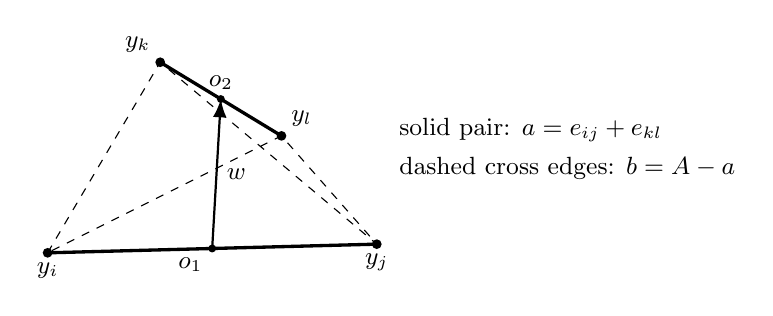
\begin{tikzpicture}[>=Latex,every node/.style={font=\small},scale=1.1]
\coordinate (a) at (-2,-.7);\coordinate (b) at (1.8,-.6);
\coordinate (c) at (-.7,1.5);\coordinate (d) at (.7,.65);
\draw[very thick] (a)--(b) (c)--(d);
\draw[dashed] (a)--(c)--(b)--(d)--(a);
\fill (a) circle(1.6pt) node[below] {$y_i$};
\fill (b) circle(1.6pt) node[below] {$y_j$};
\fill (c) circle(1.6pt) node[above left] {$y_k$};
\fill (d) circle(1.6pt) node[above right] {$y_l$};
\coordinate (o1) at ($(a)!.5!(b)$);\coordinate (o2) at ($(c)!.5!(d)$);
\fill (o1) circle(1.3pt) node[below left] {$o_1$};
\fill (o2) circle(1.3pt) node[above] {$o_2$};
\draw[->,thick] (o1)--(o2) node[midway,right] {$w$};
\node[align=left] at (4,.5) {solid pair: $a=e_{ij}+e_{kl}$\\[3pt]
 dashed cross edges: $b=A-a$};
\end{tikzpicture}
\caption{One opposite-edge partition, drawn schematically. The three such
partitions satisfy $\sum_j a_j=A$ and $\sum_j b_j=2A$. They cannot be
assigned independent worst-case deficit budgets.}\label{fig:budgets}
\end{figure}

\subsection{Exact vector relations and safe scalar bounds}
Expansion of squared distances gives
\begin{equation}\label{eq:pairgeometry}
 |w|^2=\frac12+\frac{a-b}{4},\qquad
 |k_1\cdot k_2|\le c:=\frac{b}{2(1-a)},\qquad
 |w\cdot k_i|\le\frac{b}{4\sqrt{1-a}}.
\end{equation}
Here are the cancellations behind the estimates. For $u=y_j-y_i$ and
$v=y_l-y_k$, the alternating sum of the four cross squared distances is
$\pm2u\cdot v$. The constant terms all cancel, leaving absolute value at
most $b$. Since $|u|,|v|\ge\sqrt{1-a}$, the middle inequality follows.
Differences of two cross-distance sums similarly give
$4|w\cdot u|\le b$ and $4|w\cdot v|\le b$. Finally the sum of all four
cross squared distances is
$4|w|^2+|u|^2+|v|^2$; it equals $4-b$, whereas
$|u|^2+|v|^2=2-a$. This proves the first identity.

Set
\[
 z=\frac{k_1\times k_2}{|k_1\times k_2|},\qquad w\cdot z>0,
 \qquad v_1=z\times k_1,\quad v_2=z\times k_2.
\]
The common normal $z$ exists because $c\le1/25<1$. It is not generally
parallel to $w$. The contact balance projected onto $z$ implies
$o_1\cdot z<0<o_2\cdot z$; the contacts in each pair have the same
projection, and their positively weighted average is zero.

Also $o_i\perp k_i$ and
\[
 |o_i|^2=R^2-|y_i-y_j|^2/4\ge1/8-A/16.
\]
Projecting $o_1$ onto the basis $z,v_1$, and using
$o_1\cdot k_2=-w\cdot k_2$, gives
\[
 |o_1\cdot v_1|\le\frac{b}{4\sqrt{1-a}\sqrt{1-c^2}}.
\]
The same holds for $o_2\cdot v_2$. Thus the angles between $z$ and
$-o_1/|o_1|,o_2/|o_2|$ are at most $\arcsin\eta$, where
\begin{equation}\label{eq:eta}
 \eta=\frac{b}{4\sqrt{1-a}\sqrt{1-c^2}\sqrt{1/8-(a+b)/16}}.
\end{equation}

\subsection{A common region on which both circle supports are valid}
The half-angle of each clipped circle is given by \cref{eq:phi}. On our
range its cosine increases with $s^2$ and decreases with $R$. For example,
differentiating its square with respect to $s^2$ has the sign of
$2-6R^2+R^2s^2>0$; this is positive already at the relevant endpoints.
Using $s^2\le1$ and $R^2\ge3/8-A/16$ therefore gives
\[
 \cos\beta\le C_\beta:=\sqrt{\frac4{3(2-a-b)}}.
\]
Put $S_\beta=\sqrt{1-C_\beta^2}$ and
\begin{equation}\label{eq:T}
 T(a,b)=\frac{S_\beta\sqrt{1-\eta^2}-C_\beta\eta}
              {C_\beta\sqrt{1-\eta^2}+S_\beta\eta}.
\end{equation}
This is $\tan(\arccos C_\beta-\arcsin\eta)$.
For $a,b\ge0$, $a+b\le2/25$, elementary bounds give
\begin{equation}\label{eq:Tbds}
 c\le1/25,\qquad\eta<1/16,\qquad
 \frac12<T\le\frac1{\sqrt2}<\frac34.
\end{equation}
For instance $C_\beta\le5/6$, and
$\tan(\arccos(5/6)-\arcsin(1/16))>1/2$ is checked after inserting the
radicals $\sqrt{11},\sqrt{255}$. The upper bound follows from
$\arccos C_\beta\le\arccos\sqrt{2/3}$ and $\eta\ge0$.

Use coordinates on the hemisphere $n\cdot z>0$:
\begin{equation}\label{eq:projective}
 n=\frac{z+m}{\sqrt{1+|m|^2}},\qquad m\perp z,\qquad
 x=m\cdot v_1,\quad y=m\cdot v_2.
\end{equation}
Let $\chi=k_1\cdot k_2=v_1\cdot v_2$. The Gram matrix of $v_1,v_2$ is
$\begin{psmallmatrix}1&\chi\\\chi&1\end{psmallmatrix}$. Inverting it yields
\begin{equation}\label{eq:Wchi}
 W_\chi=1+|m|^2
   =1+\frac{x^2+y^2-2\chi xy}{1-\chi^2},\qquad
 \dd\sigma=\frac{\dd x\dd y}{\sqrt{1-\chi^2}\,W_\chi^{3/2}}.
\end{equation}
The second formula combines the planar linear Jacobian
$1/\sqrt{1-\chi^2}$ with the central-projection Jacobian
$(1+|m|^2)^{-3/2}$.

Projection of $n$ into $k_1^\perp$ is proportional to $z+xv_1$, and
projection into $k_2^\perp$ to $z+yv_2$. Hence on $|x|,|y|<T$ each
projection makes angle at most $\arctan T$ with $z$. Equation \cref{eq:T}
ensures that it lies strictly inside the clipped loading arc around
$-o_1$; the antipodal projection lies inside the other arc around $-o_2$.
These points lie in the remaining two unit balls by \cref{sec:clipgeometry}.

One condition remains: a circle candidate is the support point of the
intersection of its two balls only when its normal lies in their normal
cone. In the present notation this is
\begin{equation}\label{eq:normalcone}
 |n\cdot k_i|<s_i/2.
\end{equation}
It follows either by resolving $n$ into a nonnegative combination of the
two unit normals $\pm(s_i/2)k_i+r_iv$, or by that two-dimensional cone's
half-angle. We will use the circle formulas only where a positive curvature
lower bound proves \cref{eq:normalcone}. Elsewhere the integral estimate
will use zero, so no unsupported support formula is assumed.

\subsection{Curvature on a circular edge}
For an active circle of center $o$, radius $r$, and axis $k$, the support
function on its normal region is
\[
 h(n)=o\cdot n+r\sqrt{1-(n\cdot k)^2}.
\]
Its curvature-radius matrix has eigenvalues
\begin{equation}\label{eq:circleradii}
 0,\qquad\frac r{\sqrt{1-(n\cdot k)^2}}.
\end{equation}
To verify this, take the homogeneous function
$o\cdot\xi+r\sqrt{|\xi|^2-(\xi\cdot k)^2}$ and restrict its Euclidean
Hessian to $n^\perp$. The linear term has zero Hessian; the norm of the
projection into $k^\perp$ has one nonzero tangential eigenvalue as displayed.
Complementarity gives $\Qh h_D(-n)=I-\Qh h_C(n)$, so its determinant is
one minus the nonzero radius in \cref{eq:circleradii}.

\section{The joint completion integral}\label{sec:jointintegral}
\subsection{Pairing normals removes the transverse midpoint error}
For this opposite pair let $r_1,r_2$ be its circle radii, and write
$w=w_z z+w_\perp$. Whenever both circle supports are valid,
\begin{equation}\label{eq:truegap}
 g(n)=\frac{r_1\sqrt{1+x^2}+r_2\sqrt{1+y^2}-w_z-w_\perp\cdot m}
              {\sqrt{W_\chi}}-1.
\end{equation}
The two determinants relevant to $d_*$ are
\[
 1-\frac{r_1\sqrt{W_\chi}}{\sqrt{1+x^2}},\qquad
 1-\frac{r_2\sqrt{W_\chi}}{\sqrt{1+y^2}}.
\]
Define
\[
 r_0=\sqrt{3/4},\qquad r_a=\sqrt{3/4+a/4},\qquad
 w_0=\sqrt{1/2+(a-b)/4},
\]
\begin{align}
 q_-&=\min(x^2,y^2),\qquad q_+=\max(x^2,y^2),\nonumber\\
 N&=r_0\sqrt{1+q_+}+r_a\sqrt{1+q_-}-w_0,
 &\zeta&=\frac{r_a}{\sqrt{1+q_-}}.\label{eq:Nzeta}
\end{align}
The common determinant lower bound is $1-\zeta\sqrt{W_\chi}$.
If it is positive, then
\[
 1-(n\cdot k_i)^2>r_i^2=1-s_i^2/4,
\]
which proves the required normal-cone condition \cref{eq:normalcone}.

At fixed $x^2,y^2$, the two radii obey $r_i=\sqrt{3/4+e_i/4}$ with
$e_1+e_2=a$. Their weighted sum in \cref{eq:truegap} is concave in $e_1$.
Its minimum occurs at an endpoint; the smaller endpoint pairs the larger
radius with the smaller factor. Therefore
\begin{equation}\label{eq:allocate}
 r_1\sqrt{1+x^2}+r_2\sqrt{1+y^2}
 \ge r_0\sqrt{1+q_+}+r_a\sqrt{1+q_-}.
\end{equation}
Also $w_z\le|w|=w_0$.

The square $[-T,T]^2$, the measure factor, and the determinant lower bound
are invariant under $(x,y)\mapsto(-x,-y)$. The term $w_\perp\cdot m$ is
odd under this map and cancels exactly. We do not replace it by its absolute
value. The average of the two true values of $g$ is nonnegative, since
$D\subset K$; hence its lower bound can be clamped at zero.

For fixed $N,\zeta$ define
\begin{equation}\label{eq:Phi}
 \Phi(W)=\frac{\pp{N/\sqrt W-1}\,
 q(\pp{1-\zeta\sqrt W})}{W^{3/2}}.
\end{equation}
Here $[t]_+=\max\{t,0\}$. On all values used below $W\ge1+q_+$, so
$\zeta\sqrt W\ge\sqrt3/2>4/5$. Its positive determinant argument is
therefore less than $1/5$, where $q$ is increasing and nonnegative.
Combining \cref{eq:qpoly,eq:allocate} and the antipodal pairing, the
contribution of the positive-normal square to $\int g\psi(d_*)$ is at least
\begin{equation}\label{eq:localintegral}
 \int_{[-T,T]^2}\frac{\Phi(W_\chi)}{\sqrt{1-\chi^2}}\dd x\dd y.
\end{equation}
At points with a nonpositive determinant lower bound, this expression is
zero. Their actual contribution is nonnegative, so excluding them is valid.

\subsection{Convexity averages edge obliquity}\label{sec:convexity}
\begin{lemma}\label{lem:Phi}
The function \cref{eq:Phi} is decreasing and convex for the relevant
$W\ge1+q_+$.
\end{lemma}
\begin{proof}
On the interval where both unclamped factors are positive set
\[
 G=N/\sqrt W-1,\quad D_*=1-\zeta\sqrt W,\quad
 u=\sqrt W/N\in(0,1),\quad v=\zeta\sqrt W\in[4/5,1).
\]
All three factors $G,q(D_*),W^{-3/2}$ are nonnegative and decreasing, which
proves monotonicity. For convexity write
\[
 \phi_1=GD_*W^{-3/2},\quad\phi_2=GD_*^2W^{-3/2},\quad
 \Phi=\tfrac{47}{32}\phi_1-2\phi_2.
\]
Two differentiations give $\phi_i''=NW^{-4}B_i(u,v)$, with
\[
 B_1=6-\tfrac{15}{4}(u+v)+2uv,
\]
\[
 B_2=6-\tfrac{15u}{4}-\tfrac{15v}{2}+4uv+2v^2-\tfrac34uv^2.
\]
The minimum of the bilinear $B_1$ on $[0,1]^2$ is $1/2$. The coefficient
of $u$ in $B_1/2-B_2$ is
$15/8-3v+3v^2/4<0$ for $4/5\le v\le1$. Its minimum is therefore at
$u=1$, where it equals
\[
 \frac{-9+21v-10v^2}{8}\ge\frac7{40}.
\]
Thus $\phi_2''\le\phi_1''/2$ and
$\Phi''\ge(15/32)\phi_1''>0$. Once one of the positive factors vanishes,
$\Phi$ stays zero; its derivative jumps upward to zero, preserving convexity.
If there was no positive interval, the conclusion is immediate.
Finally
$W_\chi-1-x^2=(y-\chi x)^2/(1-\chi^2)\ge0$, and likewise for $y$,
which verifies the domain used throughout.
\end{proof}

At fixed $|x|,|y|$, the two signs of $xy$ give $W_+,W_-$. Their average is
\[
 \overline W=1+\frac{x^2+y^2}{1-\chi^2}
 \le W_c:=1+\frac{x^2+y^2}{1-c^2}.
\]
Convexity and then monotonicity imply
\begin{equation}\label{eq:Jensen}
 \Phi(W_+)+\Phi(W_-)\ge2\Phi(\overline W)\ge2\Phi(W_c).
\end{equation}
As $1/\sqrt{1-\chi^2}\ge1$, \cref{eq:localintegral} is bounded below by
\begin{equation}\label{eq:F}
 \boxed{\mathcal F(a,b)=4\int_0^{T(a,b)}\int_0^{T(a,b)}
  \frac{\pp{N/\sqrt{W_c}-1}\,
       q(\pp{1-\zeta\sqrt{W_c}})}{W_c^{3/2}}\dd x\dd y.}
\end{equation}
The remaining geometric obliquity enters only through $c^2$. In contrast,
replacing $\chi xy$ by its absolute worst value in each quadrant would
introduce a first-order loss.

\subsection{Summing the three pairs without overlap}
\begin{proposition}\label{prop:joint}
For the three opposite-edge partitions and their deficits $a_j,b_j$,
\begin{equation}\label{eq:joint}
 \boxed{V_K\ge\frac{47V_D-V_C}{46}
                  +\frac8{23}\sum_{j=1}^3\mathcal F(a_j,b_j),}
\end{equation}
where
\begin{equation}\label{eq:sumbudgets}
 \sum_{j=1}^3a_j=A,\qquad\sum_{j=1}^3b_j=2A.
\end{equation}
\end{proposition}
\begin{proof}
Each positive determinant region corresponds to an interior support point
of a specified unit--unit edge of $C$. The clipped-arc and normal-cone
conditions are strict there. Distinct edges cannot share such a normal:
a finite intersection of strictly convex balls is strictly convex, so it
has a unique support point, and an interior point of the present edge has
exactly its two unit balls active. Thus these regions are disjoint except
on null boundaries. Each pair and its antipode contribute at least
$2\mathcal F(a_j,b_j)$ to the integral of \cref{eq:weighted}, proving
\cref{eq:joint}. Each of the six deficits belongs to exactly one opposite
pair, proving \cref{eq:sumbudgets}.
\end{proof}

\section{First finite certificate: the two-parameter completion integral}\label{sec:integralcert}
The first numerical premise is small in dimension: the unknown body has been
eliminated, leaving the explicit function \cref{eq:F} of two nonnegative
numbers. We state the exact rational target, then explain its verification.

\begin{lemma}[Certified affine lower bound]\label{lem:affine}
For $a,b\ge0$ and $a+b\le2/25$,
\begin{equation}\label{eq:affine}
 \boxed{\mathcal F(a,b)>L(a,b):=
 \frac{153}{100000}-\frac{601}{100000}a+\frac{317}{20000}b.}
\end{equation}
\end{lemma}

\subsection{A fixed integration square}
The integrand of \cref{eq:F} is symmetric in $x,y$. On $0\le y\le x\le T$
put $x=Ts$, $y=Tst$, with $0\le s,t\le1$. Its planar Jacobian is $T^2s$,
so
\begin{equation}\label{eq:unitintegral}
 \mathcal F(a,b)=8T^2\int_0^1\int_0^1
     s\,\Phi(W_c(Ts,Tst))\dd s\dd t.
\end{equation}
There is no minimum/maximum switch between $x^2$ and $y^2$ in these
coordinates: $x^2\ge y^2$. Define the two smooth factors
\[
 G=\frac{r_0\sqrt{1+x^2}+r_a\sqrt{1+y^2}-w_0}{\sqrt{W_c}}-1,
 \qquad D_*=1-\frac{r_a\sqrt{W_c}}{\sqrt{1+y^2}}.
\]
The complete integrand equals
$8T^2s\,[G]_+q([D_*]_+)W_c^{-3/2}$. It is nonnegative and locally
Lipschitz in the parameters. On a region where both factors are positive
it is an elementary smooth function of $a,b,s,t$ involving only rational
operations and square roots.

\subsection{Validated quadrature at a parameter center}
For fixed rational $a,b$, partition $[0,1]^2$ into $192^2$ equal cells.
A cell is retained only if directed interval arithmetic proves $G>0$ and
$D_*>0$ throughout it. All other cells are omitted. This yields a valid
lower integral because the true integrand is nonnegative.

Let $P$ denote the smooth complete integrand on a retained cell, $m$ its
center, and $h=1/384$ its half-side. The midpoint estimate is
\begin{equation}\label{eq:midpointerror}
 \frac1{|Q|}\int_Q P\ge P(m)-\frac{h^2}{6}
      \left(\sup_Q|P_{ss}|+\sup_Q|P_{tt}|\right).
\end{equation}
For clarity, in one variable Taylor's formula with integral remainder gives
$|\frac1{2h}\int_{-h}^h p(t)\,dt-p(0)|\le h^2\sup|p''|/6$.
Apply this successively to the two variables and bound each pure second
derivative on the full rectangle. No mixed derivative is required.
The right side of \cref{eq:midpointerror} is clamped below by zero, then
multiplied by the cell area and summed with downward rounding. This produces
$\underline{\mathcal F(a,b)}$.

\subsection{Control between parameter centers}
On a parameter rectangle, a separate $64^2$ interval partition in $s,t$
encloses $\mathcal F_a,\mathcal F_b$. The derivatives of $T(a,b)$ and the
Jacobian factor $8T^2s$ are included. On a cell where either positive factor
is known to be nonpositive, its derivative contribution is zero. On an
active cell one uses the ordinary smooth derivative. A possibly switching
cell uses the interval hull of zero and the smooth derivative enclosure.
This is valid almost everywhere for the locally Lipschitz positive-part
function, and hence under integration. Equivalently, apply the fundamental
theorem of calculus along a parameter segment and then Fubini's theorem.
This argument does not differentiate twice across a positive-part boundary.

For a parameter rectangle of center $m$ and half-widths $h_a,h_b$, the
acceptance test is
\begin{equation}\label{eq:paramtest}
 \underline{\mathcal F(m)}-L(m)
 -h_a\sup|\mathcal F_a-L_a|
 -h_b\sup|\mathcal F_b-L_b|>0.
\end{equation}
When it holds, the whole rectangle satisfies \cref{eq:affine}.

\subsection{Coverage and completed output}
The initial partition is the $32\times32$ dyadic tiling of $[0,2/25]^2$.
A rectangle is excluded only if its lower endpoints have sum strictly larger
than $2/25$. Otherwise it is tested by \cref{eq:paramtest}; an inconclusive
rectangle is bisected in the longer direction, with a deterministic tie rule.
The recomputation gives
\begin{center}
\begin{tabular}{@{}lr@{}}
\toprule
Accepted parameter rectangles & 584\\
Rectangles excluded by the exact triangle test & 474\\
Attempted parameter rectangles & 618\\
Maximum dyadic depth in either parameter & 6\\
Point-quadrature cells per center & $192^2$\\
Derivative-quadrature cells per rectangle & $64^2$\\
\bottomrule
\end{tabular}
\end{center}
The independent Python cover checker reconstructs the same tree. It verifies
that every accepted leaf is used exactly once and every untested leaf is
outside the triangle. Thus summing the areas is not used as a substitute
for a genuine cover check.

The least acceptance margin at 48-bit dyadic precision is
\begin{equation}\label{eq:margin48}
 \frac{17153402}{2^{48}}>0.
\end{equation}
The 52-bit recomputation gives $274686139/2^{52}>0$ and the same 584 leaves.
Both runs were completed for this manuscript. Arithmetic details and the
source-to-equation correspondence appear in \cref{sec:verification}.
These finite checks, together with the preceding error and coverage proofs,
prove \cref{lem:affine}.

\begin{corollary}\label{cor:sumaffine}
The three opposite-edge contributions satisfy
\begin{equation}\label{eq:sumaffine}
 \sum_{j=1}^3\mathcal F(a_j,b_j)>
       \frac{459}{100000}+\frac{2569}{100000}A.
\end{equation}
Consequently, for $R\ge\RS$,
\begin{equation}\label{eq:nearstructure}
 \boxed{V_K>\frac{47V_D-V_C}{46}
 +\frac8{23}\left[\frac{459}{100000}
           +\frac{2569}{100000}\,16(3/8-R^2)\right].}
\end{equation}
\end{corollary}
\begin{proof}
Sum \cref{eq:affine} and use \cref{eq:sumbudgets}:
$-601/100000+2(317/20000)=2569/100000>0$.
Then use $A\ge16(3/8-R^2)$ and \cref{eq:joint}.
\end{proof}
This calculation explains why the opposite-edge budgets must remain coupled.
They cannot all take an independent minimum of $\mathcal F$ at unrelated
values of $a,b$.

\section{Second finite certificate: the inner--outer volume combination}\label{sec:hullcert}
Define from \cref{eq:Bterms,eq:edgeterms}
\begin{equation}\label{eq:frakf}
 \mathfrak f(R,e)=\frac{47f_D(R,e)-f_C(R,e)}{46},\qquad
 H_0(R)=\frac{47B_D(R)-B_C(R)}{46}+6\mathfrak f(R,0).
\end{equation}
Then
\begin{equation}\label{eq:combination}
 \frac{47V_D-V_C}{46}
 =H_0(R)+\sum_{i<j}[\mathfrak f(R,e_{ij})-\mathfrak f(R,0)].
\end{equation}
When $R<\RJ$, the zero-deficit term $H_0(R)$ is an analytic baseline, not
the volume of a realizable regular unit tetrahedron at radius $R$.
Only the complete expression \cref{eq:combination} is applied to geometry.

\begin{lemma}[Verified derivative signs]\label{lem:hullderivs}
Throughout $\RS\le R\le\RJ$, $0\le e\le A_0$,
\begin{equation}\label{eq:derivsigns}
 H_0'(R)>0,\qquad\mathfrak f_e(R,e)>0,\qquad
 \mathfrak f_{ee}(R,e)<0,\qquad\mathfrak f_{eR}(R,e)<0.
\end{equation}
\end{lemma}

\subsection{Derivatives in a cancellation-resistant form}
The certificate checks the signs of exact derivatives, not finite
differences. Here are the expressions that make those checks practical.
Put $x=1-e$, $Q=R^2(4-x)-1$, $r=\sqrt{1-x/4}$, and
$\theta=\arcsin(\sqrt x/2)$. Keeping the angle notation from
\cref{sec:volformula}, differentiation gives
\begin{align}
 U_x&=-\frac1{\sqrt x(4-x)\sqrt Q},&
 V_x&=\frac R{\sqrt x\sqrt Q},\nonumber\\
 \Psi_x&=-\frac{R(1-2R^2)}{\sqrt x(4R^2-x)\sqrt Q},&
 \phi_x&=\frac{2(6R^2-R^2x-2)}{(4-x)(4R^2-x)\sqrt Q},\label{eq:anglederivs}\\
 (T_e)_x&=\frac{4R^2-1-2R^2x}{2\sqrt x\sqrt Q},&
 F_x&=-\frac{\sqrt x}{16}+\frac{\theta}{8r}.\nonumber
\end{align}
For example, differentiate each cosine, use
$(\arccos z)'=-z'/\sqrt{1-z^2}$, and simplify by
$4r^2m^2-(1-x/2)^2=Q$. Each denominator is positive on the rectangle.
Substitution into \cref{eq:edgeterms} cancels the larger angle derivatives
and gives
\begin{equation}\label{eq:outerdx}
 \partial_x f_C(R,1-x)=
 \frac{(2-x)\sqrt Q}{4\sqrt x(4R^2-x)}
 -\frac{(4-x)\phi}{16\sqrt x},
\end{equation}
\begin{align}\label{eq:innerdx}
 \partial_x f_D(R,1-x)={}&
 \phi\left(-\frac{\sqrt x}{16}+\frac{\theta}{8r}\right)
 +\frac{(x+6-8R)\sqrt Q}{4\sqrt x(4R^2-x)}\notag\\
 &-\frac{(6R^2-R^2x-2)\theta}{\sqrt{4-x}\sqrt Q(4R^2-x)}
 -\frac{\sqrt{4R^2-1}(1-2R^2)\gamma}{\sqrt x\sqrt Q(4R^2-x)}.
\end{align}
The code differentiates the combination of these expressions in $x$ and
$R$. Recall $\partial_e=-\partial_x$: hence the three required edge signs
are equivalent to $\mathfrak f_x<0$, $\mathfrak f_{xx}<0$,
$\mathfrak f_{xR}>0$ in the $x$ notation.

\subsection{The complete derivative cover}
Divide $[\RS^2,3/8]$ into 32 rational intervals and $[0,A_0]$ into 100
rational intervals. Taking an outward square root in the first coordinate
gives 3,200 boxes in $(R,e)$. On each box the program encloses
\cref{eq:outerdx,eq:innerdx} and the exact first derivatives of their
combination. It also encloses $H_0'$ on all 32 radius intervals. All four
strict comparisons in \cref{eq:derivsigns} pass at both 128-bit and 192-bit
fixed-dyadic precision. Every radical and inverse-trigonometric argument
range is checked before evaluation. This proves \cref{lem:hullderivs}
subject only to the explicit arithmetic implementation described below.

\subsection{Turning the signs into a six-edge estimate}
The positive, concave edge increments can be bounded by secants; no
optimization over the six edge lengths remains. Partition
$[\RS^2,3/8]$ into 512 consecutive rational intervals
$[z_j,z_{j+1}]$. Put
\[
 d_j=3/8-z_j,\qquad E_j=\frac{16d_j}{1-8d_j},\qquad
 m_j=\frac{\mathfrak f(\sqrt{z_{j+1}},E_j)
              -\mathfrak f(\sqrt{z_{j+1}},0)}{E_j}>0.
\]
Each $E_j>0$, including the last interval's left endpoint. For
$\sqrt{z_j}\le R\le\sqrt{z_{j+1}}$, the contact budget gives $0\le e_{ij}\le E_j$.
Since $\mathfrak f_{eR}<0$, integrating in $e$ first gives
\[
 \mathfrak f(R,e)-\mathfrak f(R,0)
 \ge\mathfrak f(\sqrt{z_{j+1}},e)-\mathfrak f(\sqrt{z_{j+1}},0).
\]
Concavity in $e$ bounds the latter below by its chord $m_je$. Hence
\[
 \frac{47V_D-V_C}{46}
 \ge H_0(\sqrt{z_j})+m_j A
 \ge H_0(\sqrt{z_j})+16d_{j+1}m_j.
\]
Combining with \cref{eq:nearstructure}, every body in that interval satisfies
\begin{equation}\label{eq:bucket}
 V_K>H_0(\sqrt{z_j})+16d_{j+1}m_j
 +\frac8{23}\left[\frac{459}{100000}
       +\frac{2569}{100000}\,16d_{j+1}\right].
\end{equation}

The 512 right sides are evaluated with directed intervals and compared
with $259/625$ by integer arithmetic. At 128-bit precision the smallest
lower endpoint is
\begin{equation}\label{eq:nearminimum}
 \frac{141028929484742528892496879275454481331}{2^{128}}
 >0.4144467>\frac{259}{625}.
\end{equation}
The 192-bit run verifies the same strict target. Thus the complete
near-Jung range is controlled. Neither a sampled tetrahedron nor an assumed
worst symmetric configuration enters this conclusion.

\section{A radial inequality for the complementary circumradii}\label{sec:radial}
We now give the other branch of the proof. The method is due to Hyra
\cite{Hyra}; it is derived here to specify exactly what the rational
certificate must verify. In this section assume temporarily that $\partial K$
is $C^1$. The last section removes this assumption.

\subsection{Radial function and the opposite-point inequality}
Since $(1-R)B\subset K$, define the continuous radial function
\[
 \rho(u)=\max\{t\ge0:tu\in K\},\qquad 1-R\le\rho(u)\le R.
\]
Polar coordinates give
\begin{equation}\label{eq:radialvol}
 3V_K=\int_{\Sph}\rho(u)^3\dd\sigma(u).
\end{equation}
At a boundary point $x$ with outward unit normal $n$, \cref{lem:width}
gives $x-n\in K\subset RB$. Squaring gives
\begin{equation}\label{eq:radialnormal}
 2x\cdot n\ge |x|^2+1-R^2.
\end{equation}
Take $0<m\le1-R^2$ and the radial vector field
$F_m(x)=2x/(|x|^2+m)$. Its boundary flux obeys $F_m(x)\cdot n\ge1$,
so the divergence theorem yields
\[
 S_K\le\int_K\operatorname{div}F_m\dd x.
\]
At radius $r$, $\operatorname{div}F_m=2(r^2+3m)/(r^2+m)^2$. The radial
integral is explicit because
\[
 \frac{d}{dr}\frac{2r^3}{r^2+m}
   =\frac{2r^2(r^2+3m)}{(r^2+m)^2}.
\]
Therefore
\begin{equation}\label{eq:radialarea}
 S_K\le\int_{\Sph}\frac{2\rho^3}{\rho^2+m}\dd\sigma.
\end{equation}

\subsection{A tangent majorant and its recoverable deficit}
Let $s_0>0$ and define
\begin{align}
 a&=\frac{2(s_0^2+3m)}{3(s_0^2+m)^2},&
 b&=\frac{2s_0^3}{s_0^2+m}-as_0^3,\nonumber\\
 G(s)&=as^3+b-\frac{2s^3}{s^2+m}.\label{eq:tangent}
\end{align}
These constants are the slope and intercept of the tangent line at
$X=s_0^3$ to $\phi(X)=2X/(X^{2/3}+m)$. Direct differentiation gives
\[
 \phi''(X)=-\frac{4(X^{2/3}+5m)}{9X^{1/3}(X^{2/3}+m)^3}<0.
\]
Thus $G(s)\ge0$, with equality only at $s=s_0$. Also $G$ decreases below
$s_0$ and increases above $s_0$, since its derivative has the sign of
$\phi'(s_0^3)-\phi'(s^3)$.
Using \cref{eq:radialvol,eq:radialarea} and Blaschke's identity gives
\[
 2V_K+2\pi/3\le3aV_K+4\pi b-\int G(\rho)\dd\sigma.
\]
Whenever $3a-2>0$,
\begin{equation}\label{eq:master}
 \boxed{V_K\ge
 \frac{2\pi/3-4\pi b+\int_{\Sph}G(\rho)\dd\sigma}{3a-2}.}
\end{equation}
The aim of the cap construction is to retain a positive portion of the last
integral, rather than discard it everywhere.

For $R\le3/5$, choose $m=16/25$ and $s_0=37/80$ and discard it. The
conditions $m\le1-R^2$ and $3a-2>0$ hold. Exact rational simplification yields
\begin{equation}\label{eq:lowradius}
 V_K\ge\frac{76439431}{575385750}\pi
       >0.4173574>\frac{259}{625}.
\end{equation}
It remains to cover $3/5\le R\le\RS$.

\subsection{Angular separation of the four contacts}
For a radius interval $R_-\le R\le R_+$ in this range, put
\[
 \eta=\frac1{2R_-^2}-1.
\]
The contact directions $u_i=y_i/R$ obey $u_i\cdot u_j\ge-\eta$.
They also obey the upper bound
\begin{equation}\label{eq:contactupper}
 u_i\cdot u_j\le T_*:=\frac{4\eta^2}{1-\eta}-1.
\end{equation}
For a proof, let $t=u_1\cdot u_2$ and $A'=\lambda_1+\lambda_2$.
Dot the balance equation with $u_1,u_2$ separately, replace cross scalar
products by their lower bound, and add:
\[
 A'(1+t)\le2\eta(1-A').
\]
For the other two labels the same estimate, using their mutual scalar
product at least $-\eta$, gives
$(1-A')(1-\eta)\le2\eta A'$. Thus
$A'\ge(1-\eta)/(1+\eta)$. Substitution proves
\cref{eq:contactupper}. Taking the larger $\eta$ from $R_-$ weakens the
bound and makes it valid on the whole radius interval.

\subsection{Upper radial bounds near the negative contact directions}
If $u$ is at angle $\theta<\pi/2$ from $-u_i$, the points $\rho(u)u$ and
$Ru_i$ have distance at most one. Hence
\[
 \rho(u)^2+2R\cos\theta\,\rho(u)+R^2\le1.
\]
Replacing $R$ by $R_-$ decreases the left side. Its positive root gives
\begin{equation}\label{eq:negativecap}
 \rho(u)\le\Pi(R_-,\cos\theta):=
       -R_-\cos\theta+\sqrt{1-R_-^2\sin^2\theta}.
\end{equation}
This upper bound increases with $\theta$. Therefore a bound at the outer
edge of a cap also bounds all its inner directions.

\subsection{Lower radial bounds propagated from the positive contacts}
Set $m=1-R_+^2$ for the radius interval. The normal-angle inequality
\cref{eq:radialnormal} says that, at a point of radial value $s$, its outward
normal makes angle at most
\[
 \gamma_m(s)=\arccos\frac{s^2+m}{2s}
\]
with the radial direction. This is real on the actual radial range and
increases with $s$, since $s^2\le R^2<m$.

Suppose two directions $u,u'$ are separated by angle $\delta$ and the normal
at $s u'$, $s=\rho(u')$, makes angle $\gamma$ with $u'$. Its supporting plane
gives
\[
 \rho(u)\le\frac{s\cos\gamma}{\cos(\gamma+\delta)}
\]
when $\gamma+\delta<\pi/2$. The ratio on the right increases with $\gamma$;
its derivative is $\sin\delta/\cos^2(\gamma+\delta)$. Consequently
\begin{equation}\label{eq:N}
 \rho(u)\le N_m(\rho(u'),\delta),\qquad
 N_m(s,\delta)=\frac{s(s^2+m)}{(s^2+m)\cos\delta
 -\sqrt{4s^2-(s^2+m)^2}\sin\delta}.
\end{equation}
This function increases with $s$ and with $\delta$ wherever the denominator
is positive. For the first assertion, rewrite it as
$[(s^2+m)/2]/\cos(\gamma_m(s)+\delta)$; both factors increase with $s$.

Thus, if $N_m(X,\delta)\le Y$ and the radial value at one direction is at
least $Y$, then the radial value at a direction within $\delta$ is at least
$X$. Otherwise monotonicity applied to \cref{eq:N} would give a strict
contradiction. Beginning at $\rho(u_i)=R\ge R_-$ propagates lower bounds
outward from every positive contact.

\subsection{A rational grid makes every propagation test algebraic}
Choose $N=4096$ and use
\begin{equation}\label{eq:anglesgrid}
 \theta_k=2\arctan(k/N),\quad
 c_k=\frac{N^2-k^2}{N^2+k^2},\quad s_k=\frac{2Nk}{N^2+k^2}.
\end{equation}
These are exact rational cosines and sines. For
$\delta_k=\theta_k-\theta_{k-1}$, angle subtraction gives rational
$c_k^\Delta,s_k^\Delta$ as well.

Let $X,Y>0$ be rational candidates and put $T=X^2+m$,
$D_*=4X^2-T^2$. The three rational inequalities
\begin{equation}\label{eq:steptest}
 D_*\ge0,\qquad Yc_k^\Delta-X>0,\qquad
 Y^2D_*(s_k^\Delta)^2\le T^2(Yc_k^\Delta-X)^2
\end{equation}
prove $N_m(X,\delta_k)\le Y$ and positivity of its denominator.
Indeed, both sides being nonnegative, take the square root of the last
inequality to get
$Y\sqrt{D_*}s_k^\Delta\le T(Yc_k^\Delta-X)$.
Rearranging gives
$T c_k^\Delta-\sqrt{D_*}s_k^\Delta\ge TX/Y>0$, as required.

A decreasing sequence $w_0=R_-,w_1,\ldots,w_{n_+}>s_0$ passing
\cref{eq:steptest} with $X=w_k,Y=w_{k-1}$ proves
\begin{equation}\label{eq:positivecert}
 \rho(u)\ge w_k\quad\text{for }d(u,u_i)\le\theta_k.
\end{equation}
Induction along a shortest great-circle segment proves this also for points
strictly inside each cap, since a previous point can be chosen at distance
at most $\delta_k$ and inside the preceding cap.

For negative caps, a rational $z_k\le s_0$ is an upper bound at angle
$\theta_k$ whenever
\begin{equation}\label{eq:ztest}
 z_k+R_-c_k\ge0,\qquad
 (z_k+R_-c_k)^2\ge1-R_-^2s_k^2.
\end{equation}
The first sign makes taking a square root legitimate, so \cref{eq:ztest}
implies $z_k\ge\Pi(R_-,c_k)$. Equation \cref{eq:negativecap} then applies
throughout the cap.

\subsection{Disjoint caps and the integrated deficit}
Require $n_+,n_-<N$ and
\begin{equation}\label{eq:disjoint}
 c_{n_+}^2-s_{n_+}^2>T_*,\qquad
 c_{n_-}^2-s_{n_-}^2>T_*.
\end{equation}
The half-angles are below $\pi/2$, and \cref{eq:contactupper,eq:disjoint}
ensure that distinct positive caps are disjoint, as are distinct negative
caps. A positive cap and a negative cap cannot meet: their radial inequalities
would give both $\rho>s_0$ and $\rho\le s_0$ there.

The spherical ring $\theta_{k-1}\le d(u,u_i)\le\theta_k$ has area
$2\pi(c_{k-1}-c_k)$. On a positive ring,
$G(\rho)\ge G(w_k)$, and on a negative ring $G(\rho)\ge G(z_k)$, by the
monotonicities following \cref{eq:tangent}. The remaining directions
contribute nonnegatively. Thus, defining
\[
 \Delta=4\sum_{k=1}^{n_+}(c_{k-1}-c_k)G(w_k)
       +4\sum_{k=1}^{n_-}(c_{k-1}-c_k)G(z_k),
\]
we have $\int G(\rho)\ge2\pi\Delta$. The resulting bound is
\begin{equation}\label{eq:capfinal}
 \boxed{V_K\ge\pi\frac{2/3-4b+2\Delta}{3a-2}.}
\end{equation}
This is the sole numerical radial expression checked in the next section.

\section{Third finite certificate: the radial intervals}\label{sec:radialcert}
The eight consecutive intervals below cover $[3/5,\RS]$ exactly. Every
number in the first three columns is a terminating decimal interpreted as
an exact rational. In every row $N=4096$, and all candidates $w_k,z_k$
are integer multiples of $10^{-12}$ stored in
\path{verification/data/radial_candidates.json}.
\begin{center}\small
\begin{tabular}{@{}cccrrr@{}}
\toprule
$R_-$ & $R_+$ & $s_0$ & $n_+$ & $n_-$ & Lower endpoint, approximately\\
\midrule
.60000 & .60500 & .479322 & 796 & 1675 & .416450260822\\
.60500 & .60700 & .485500 & 758 & 1794 & .415235053685\\
.60700 & .60800 & .489000 & 735 & 1850 & .414578330679\\
.60800 & .60825 & .492000 & 714 & 1889 & .414557800923\\
.60825 & .60840 & .492500 & 711 & 1897 & .414452404230\\
.60840 & .60845 & .492900 & 708 & 1902 & .414436432226\\
.60845 & .608475 & .493000 & 707 & 1903 & .414421400194\\
.608475 & .60849 & .493000 & 707 & 1904 & .414410955179\\
\bottomrule
\end{tabular}
\end{center}

The checker verifies the endpoint partition, $m=1-R_+^2$, $3a-2>0$, the
strict ordering and ranges of the candidates, every inequality in
\cref{eq:steptest,eq:ztest}, and both disjointness comparisons in
\cref{eq:disjoint}. These tests are rational inequalities. No trigonometric
function is numerically evaluated on the angular grid.

Each nonnegative ring contribution to $\Delta$ is rounded downward to an
integer multiple of $10^{-18}$ before summation. This weakens the bound in
the correct direction. The rational coefficient of $\pi$ in
\cref{eq:capfinal} is positive. We use the independently proved lower bound
\begin{equation}\label{eq:pi40}
 \pi_{40}=6\sum_{k=0}^{39}
       \frac{\binom{2k}{k}}{(2k+1)2^{4k+1}}<\pi.
\end{equation}
It is the first 40 terms of the positive series $6\arcsin(1/2)=\pi$.
Multiplying by $\pi_{40}$ gives a rational volume lower bound. Every one of
the eight results exceeds $259/625$ by integer cross-multiplication.
The same rational lower bound for $\pi$ verifies \cref{eq:lowradius}.

The full rational result is stored in the machine-readable report. For a
short exact bound suitable for the text, that result is strictly greater than
\begin{equation}\label{eq:radialmin}
 \frac{4144109}{10000000}=0.4144109>\frac{259}{625}.
\end{equation}
The full endpoint is approximately $0.41441095517972193$. The additional
comparison with the compact rational in \cref{eq:radialmin} is checked by
integer cross-multiplication in the manuscript audit script.
The rational candidates may originally be proposed by floating-point search,
but the default verification does not run that search and does not trust
it. An inaccurate candidate fails an exact test rather than being accepted
on the basis of its origin.

\section{Assembly for all constant-width bodies}\label{sec:assembly}
\begin{proof}[Proof of \cref{thm:main}]
For a width-one body with $C^1$ boundary, choose its minimum circumsphere.
If $R\le3/5$, use \cref{eq:lowradius}. If $3/5\le R\le\RS$, use the eight
radial certificates. If $\RS\le R\le\RJ$, use
\cref{eq:bucket,eq:nearminimum}. These ranges cover every possible
circumradius. Every branch has a fixed positive margin above $259/625$,
and there are finitely many final radius intervals. In particular the
smallest certified value is the full radial endpoint bounded below in \cref{eq:radialmin}.

For an arbitrary width-one convex body set
\[
 K_\epsilon=\frac{K+\epsilon B}{1+2\epsilon},\qquad\epsilon>0.
\]
It has width one. The boundary of $K+\epsilon B$ is $C^1$: its outward normal
is the normalized displacement from its unique nearest point in the closed
convex set $K$, and nearest-point projection is continuous. Thus the first
part applies to every $K_\epsilon$. These bodies converge in Hausdorff
distance, and hence in volume, to $K$. The fixed positive margin above
$259/625$ survives the limit. Finally, dilation by $w$ multiplies volume by
$w^3$, giving \cref{eq:main}.
\end{proof}

Notice that the word ``strict'' in \cref{eq:main} is not inferred merely from
a sequence of strict inequalities. It follows from the uniform quantitative
margin of the finite assembly. The numerical estimates are not asserted to
be attained by any body.

\section{Arithmetic, reproducibility, and the role of the computer}\label{sec:verification}
\subsection{What is a premise and what is not}
The finite premises of the theorem are exactly:
\begin{center}
\begin{tabular}{@{}p{.48\textwidth}p{.43\textwidth}@{}}
\toprule
Finite statement & Mathematical justification for its use\\
\midrule
The affine bound \cref{eq:affine} & Validated quadrature, parameter derivative
bounds, and the complete cover in \cref{sec:integralcert}.\\[4pt]
The derivative signs and 512 values in \cref{sec:hullcert} & The exact edge
formulas and the secant argument, applied to the contact budget.\\[4pt]
The eight rational radial rows & The propagation, sign, disjointness, and
ring-integration implications in \cref{sec:radial}.\\
\bottomrule
\end{tabular}
\end{center}
The programs do not prove the normal-cone lemma, the clipped boundary
incidence, the geometric support-region statements, or the mixed-volume
identities. Those are the analytic parts proved in this manuscript. Conversely,
no unproved numerical optimization statement is used in those analytic
arguments. This separation makes the computer-assisted claim auditable.

\subsection{Fixed-dyadic intervals}
At precision $b$, an interval is represented as $2^{-b}[L,U]$ with integer
endpoints. To enclose a rational $p/q$, use the floor and ceiling of
$2^bp/q$. Addition and subtraction of interval endpoints are exact integer
operations. For multiplication compute all four integer endpoint products,
take their minimum and maximum, divide by $2^b$, and round outward. An
interval containing zero cannot be inverted. On an interval of one strict
sign, the reciprocal is decreasing, so its endpoints are obtained from
$2^{2b}/U$ and $2^{2b}/L$ with outward rounding.

A square crossing zero has lower endpoint zero and upper endpoint the larger
squared endpoint, rounded upward. For square roots, the lower integer
endpoint is the integer square root of $L2^b$; the upper is the integer
square root of $U2^b$, increased by one unless its square is exact.
These rules are inclusion-preserving by elementary order properties.
Any negative radicand or zero denominator stops verification.

The Python hull arithmetic uses arbitrary-size integers at $b=128$ and
$b=192$. The C++ integral arithmetic uses 64-bit endpoints at $b=48$ and
$b=52$, with all products in signed 128-bit integers. A product of signed
64-bit integers fits in signed 128 bits; every conversion back to 64 bits
is range-checked. The square-root routine uses a floating root only as an
initial integer proposal, then corrects it until exact integer inequalities
prove the lower and upper endpoints. No floating-point sign comparison is
used to accept a cell.

\subsection{Derivative enclosures}
A derivative jet stores a function value and its first and second derivatives
as intervals. Addition, multiplication, and composition propagate the exact
rules, for example
\[
 (fg)'=f'g+fg',\quad (fg)''=f''g+2f'g'+fg'',
\]
\[
 (\phi(f))'=\phi'(f)f',\qquad
 (\phi(f))''=\phi''(f)(f')^2+\phi'(f)f''.
\]
The integral checker carries two pure second derivatives because
\cref{eq:midpointerror} does not require a mixed derivative. The hull
checker differentiates the analytic derivative expressions
\cref{eq:outerdx,eq:innerdx}. It does not differentiate a table of sampled
values or a finite difference approximation.

\subsection{Enclosing the inverse trigonometric functions}
The hull formulas require inverse trigonometric values. For $0\le x<7/10$
we use
\[
 \arcsin x=\sum_{n=0}^\infty a_nx^{2n+1},\qquad
 a_n=\frac{\binom{2n}{n}}{4^n(2n+1)}.
\]
The coefficients decrease. After retaining $n=0,\ldots,48$, the positive
tail is at most $a_{48}x^{99}/(1-x^2)$. Monotonicity encloses interval
arguments by enclosing their endpoints. For $0\le x<1/2$, the alternating
arctangent series through $x^{81}/81$ has its remainder between
$-x^{83}/83$ and zero. Machin's identity
\[
 \pi=16\arctan(1/5)-4\arctan(1/239)
\]
therefore gives an independent interval for $\pi$.

When an arccosine argument is near one, the implementation uses
\[
 \arccos x=2\arctan\sqrt{\frac{1-x}{1+x}}.
\]
Otherwise it uses $\pi/2-\arcsin x$, with signs handled explicitly.
All argument ranges are checked. Derivatives use the exact formulas
$(\arcsin x)'=(1-x^2)^{-1/2}$ and
$(\arcsin x)''=x(1-x^2)^{-3/2}$, and their arctangent counterparts,
not derivatives of an uncontrolled truncated series.

The small edge function $F$ in \cref{eq:smallF} is evaluated without
subtraction of nearly equal numbers. With $x=s/2$ it has the positive series
\begin{equation}\label{eq:Fseries}
 F(s)=\sum_{n=1}^\infty\frac{\beta_n}{2n+3}x^{2n+3},\qquad
 \beta_0=1,\quad \beta_n=\frac{2n}{2n+1}\beta_{n-1}.
\end{equation}
For a derivation differentiate
$x-x^3/3-\sqrt{1-x^2}\arcsin x$; the derivative is
$\sum_{n\ge1}\beta_n x^{2n+2}$. Integrate from zero.
The checker retains $n=1,\ldots,34$. The first omitted power is $s^{73}$.
For the value and its first two $s$-derivatives, the ratio between subsequent
positive terms is bounded above by
\[
 \frac{s_+^2}{4}\frac{75\cdot74}{73\cdot72}<1.
\]
A geometric-series bound encloses all three tails. The jet chain rule then
includes the derivatives of $s$ with respect to the chosen variable.

\subsection{The files and commands}
The directory \path{verification/} contains all source files and finite
input data. Its principal correspondence with this proof is:
\begin{center}\small
\begin{tabular}{@{}p{.38\textwidth}p{.53\textwidth}@{}}
\toprule
File & Purpose\\
\midrule
\path{projective_certificate.cpp} & \cref{eq:unitintegral,eq:midpointerror,eq:paramtest}
and the adaptive parameter certificate.\\[3pt]
\path{verify_auxiliary.py} & Geometric constants, the independent cover check,
and assembly of radial rows.\\[3pt]
\path{clipped_hull.py}, \path{combined_hull.py} &
\cref{eq:edgeterms,eq:frakf,eq:outerdx,eq:innerdx}.\\[3pt]
\path{verify_weighted_hull.py} & 3,200 derivative boxes and 512 secant lower bounds.\\[3pt]
\raggedright\path{cap_certificate.py},\newline \path{data/radial_candidates.json} &
All rational propagation and cap data.\\[3pt]
\path{interval.py}, \path{analytic_functions.py} &
Directed interval and derivative operations and rigorous series tails.\\[3pt]
\path{verify_regular_endpoint.py} & Regular tetrahedral specialization and constants.\\[3pt]
\path{verify.py} & Full execution and the exact final comparison.\\
\bottomrule
\end{tabular}
\end{center}
From that directory run
\begin{verbatim}
python verify.py --output reports/recheck_48_128
python verify.py --cpp-bits 52 --interval-bits 192 \
    --output reports/recheck_52_192
\end{verbatim}
The requirements are Python 3 and a C++17 compiler supporting signed 128-bit
integers, such as \texttt{g++}. No third-party Python package is needed for
these two commands. They recompile the checker, recompute all cell bounds,
reconstruct the cover independently, verify all radial data, and record exact
lower endpoints and SHA-256 hashes. Stored reports are not used as numerical
premises. Verification refuses Python's optimization flag \texttt{-O}, which
would disable assertions.

Both complete commands were executed in preparing this manuscript. Their
reports are supplied in \path{reports/run_48_128/} and
\path{reports/run_52_192/}. They agree on the cover and pass all required
inequalities. These are two precisions of the same implementation, not two
independently developed mathematical implementations. The result has not
been formalized in a proof assistant or independently peer-reviewed.

\section{The remaining sharp gap}\label{sec:remaining}
For exact regular tetrahedral contacts, $R=\RJ$ and all deficits vanish.
The clipping disappears. Put $\alpha=\arccos(1/3)$. The formulas above give
\[
 V_C=V_R=\frac{8\pi}{3}+\frac{\sqrt2}{4}-\frac{27\alpha}{4},
 \qquad V_D=2\VM-V_R.
\]
They can be obtained directly by setting the collapsed unit--$R$ edge sum
to zero in the surface and volume formulas. At regularity,
$S_C=8\pi-18\alpha$ and
$M_C-S_C=(\pi\sqrt3/2)\alpha$, which also verify the dual-volume identity.
Using $A=0$ in \cref{eq:nearstructure} yields the rigorous specialization
\begin{equation}\label{eq:regularbound}
 V_K\ge\frac{47(2\VM-V_R)-V_R}{46}+\frac{459}{287500}
 >0.4190589
\end{equation}
for every width-one body containing the regular unit tetrahedron. Such a
body necessarily has $R=\RJ$: the tetrahedron already has that circumradius,
and \cref{eq:weightbound} supplies the reverse inequality.

This value remains below $\VM$. Universally, \cref{thm:main} gives only
\[
 0.4144<\inf_{\operatorname{width}(K)=1}V_K
               \le0.419860045965080\ldots.
\]
The relative difference is about $1.30044\%$ of $\VM$.

The steps that lose sharpness are explicit. The weighted completion estimate
minimizes a curvature expression without retaining the differential relation
between that curvature and the support increment. The polynomial minorant
and restricted circle-support regions weaken it further. The affine bound
for $\mathcal F$ introduces another numerical loss, although it correctly
retains the three coupled budgets. The radial branch also uses a tangent
majorant and recovers its deficit only on selected caps. None of these
estimates is claimed to be equality-sensitive at a Meissner body.

A proof of the sharp value must repair these losses or replace the
corresponding estimates. Improving a finite decimal comparison, by itself,
is not such a proof. In particular, no inclusion monotonicity conjecture for
Meissner generators and no conjectural minimization over tetrahedron-containing
bodies is used in the theorem above.

\clearpage
\appendix
\section{Notation at a glance}
\begin{longtable}{@{}p{.24\textwidth}p{.67\textwidth}@{}}
\toprule
Symbol & Meaning\\\midrule\endhead
$K,w,R$ & Unknown constant-width body, its width, and normalized minimum circumradius.\\
$B,\B(E)$ & Unit ball and intersection of unit balls centered at $E$.\\
$Y=\{y_i\}$ & Four positively balanced circumsphere contacts.\\
$e_{ij},A,d$ & Squared-edge deficits, their sum, and $3/8-R^2$.\\
$C,D$ & Clipped outer body $RB\cap\B(Y)$ and its unit-ball transform.\\
$V_E,S_E,M_E$ & Volume and the two nonconstant Steiner coefficients.\\
$h_E,\Qh h_E$ & Support function and curvature-radius matrix.\\
$f,g$ & Support increment $h_K-h_D$ and missing width $1-h_D(n)-h_D(-n)$.\\
$\cA,\cH$ & Curvature matrices of $D$ and $K$, not the scalar deficit $A$.\\
$s,r,m$ & One contact edge length, its loading-circle radius, and midpoint distance.\\
$\phi,U,V,\Psi$ & The four edge angles defined in \cref{sec:volformula}.\\
$a,b$ & Opposite-edge and cross-edge deficit sums for one partition.\\
$\chi,c,\eta,T$ & Actual edge cosine, its bound, midpoint tilt bound, and projective cutoff.\\
$x,y,W_\chi$ & Common-normal projective coordinates and their normalization factor.\\
$\mathcal F,L$ & Explicit completion integral and its certified affine lower bound.\\
$\mathfrak f,H_0$ & Weighted one-edge volume term and zero-deficit analytic baseline.\\
$\rho,m,s_0,a,b,G$ & Radial function and tangent-majorant data; the last four scalar
symbols are local to \cref{sec:radial,sec:radialcert}.\\
\bottomrule
\end{longtable}

\begin{thebibliography}{9}
\bibitem{Schneider}
R.~Schneider, \emph{Convex Bodies: The Brunn--Minkowski Theory},
second expanded edition, Encyclopedia of Mathematics and its Applications,
vol.~151, Cambridge University Press.
\href{https://doi.org/10.1017/CBO9781139003858}{doi:10.1017/CBO9781139003858}.

\bibitem{Hyra}
Hyra, \emph{A certified geometric lower bound for the three-dimensional
Blaschke--Lebesgue problem}, posted 15 August 2026,
Tencent-Hunyuan/Hyra-results, mathematical manuscript and certificate.
\url{https://github.com/Tencent-Hunyuan/Hyra-results/tree/main/AI4Science/3d_blaschke_lebesgue}.
The radial construction is rederived and its required rational data are
verified in this manuscript's accompanying package.

\bibitem{HyndVolume}
R.~Hynd, \emph{The perimeter and volume of a Reuleaux polyhedron},
Journal of Computational Geometry \textbf{16}(1) (2025), 35--64.
\href{https://doi.org/10.20382/v16i1a2}{doi:10.20382/v16i1a2};
\href{https://arxiv.org/abs/2310.08709}{arXiv:2310.08709}.

\bibitem{Bogosel}
B.~Bogosel, \emph{Dangling points in area-minimizing Meissner polyhedra},
\href{https://arxiv.org/abs/2608.19747}{arXiv:2608.19747} (2026).
The conjectures discussed there are not assumptions of this proof.
\end{thebibliography}
\end{document}
